\chapter{Results}
\label{chapter:results}
In this chapter the result of the current implementation will be presented and discussed in details to have an insight of the important observable issues. Trying to tackle the different schemes and naturally compare it to a full grid method is the primary objective here. \\

%%%The problem at hand might seem very trivial at first as the interpolation problem is being investigated in two dimensions. However, the flexibility and robustness of the implementation shows how it can easily be extended to the higher dimension. It is also how a complex data structure has been implemented to give a proper base for future works.\\

In addition, not only the solution at hand is the base for higher dimension, it can also be a base for different applications, such as regression and data fitting problem in data mining, preconditioner for multigrid-like methods, partial differential equation solver in elliptic and parabolic problems, and more importantly in computational mechanics, chemistry or physics. However, by realizing this hierarchy of complexity of problems, it can be observed that interpolation problem is the fundamental method which is the task discussed here. The author acknowledges the drawbacks of method mainly in regard to convergence, but also addresses the reasons which could resolve a part of those problems for the current implementation.\\

As discussed earlier in chapter \ref{chapter:myImplementation}, the objective here is to project the result of the combination technique to the full grid. This has already been done by the fact that the underlying idea of the current implementation is to first project the function values of different level vector grids all to be combined with into a corresponding full grid and then combine them pointwise. This way some advantages and some disadvantage compared to other combination schemes presented in the literature can be observed. \\

Firstly, the obvious disadvantage would be the fact that by projection of all grids to a full grid requires a lot of extra memory consumption and this is exactly against the idea of rectifying curse of dimensionality. However, a solution is described here to address this problem, which will be better observed after the examination of the results of the adaptive refinement strategy. Assuming the method works for the adaptive refinement, it gives the rise to idea that it is required to use a coarse grid and use adaptive refinement in the areas needed. This way, total error of same order will be achieved with less storage and operations in comparison to full grid which needs high resolution in the first place. In the worst case scenario, the full grid resolution will be achieved and the solution structure requires exactly the number of grids in combination technique scheme multiplied by the storage required for the normal full grid. Since high valued level vector is not used in this case, it is not a significant weakness.\\

In contrast, the advantage that can be achieved in this method is that while the required tasks performed separately for each of the grids in the implemented version of combination method is same as normal combination technique, the extra effort is just from a projection. Therefore, using a very efficient projection method, there are not many operations added to the solution which ultimately means less computational effort compared to solution on normal full grid method. Another advantage of this, as discussed earlier, can be possibility to start with a coarse grain solution and adaptively refine to areas needed. A detailed investigation of using lower resolution schemes for lower subtree problems can possibly show better result for storage space and memory usage. \\

Note that conventionally we are using the unit square domain as shown in figure \ref{fig:results1Square}. The reason for this is that mathematically, the division of square domain is easier and straightforward. However, our implementation can work with any rectangular domain as shown in an example in figure \ref{fig:results1Rect}. 

%1figure rectangle and figure square together
\begin{figure}[h]
	\centering
    \begin{subfigure}[b]{0.49\textwidth}    
	    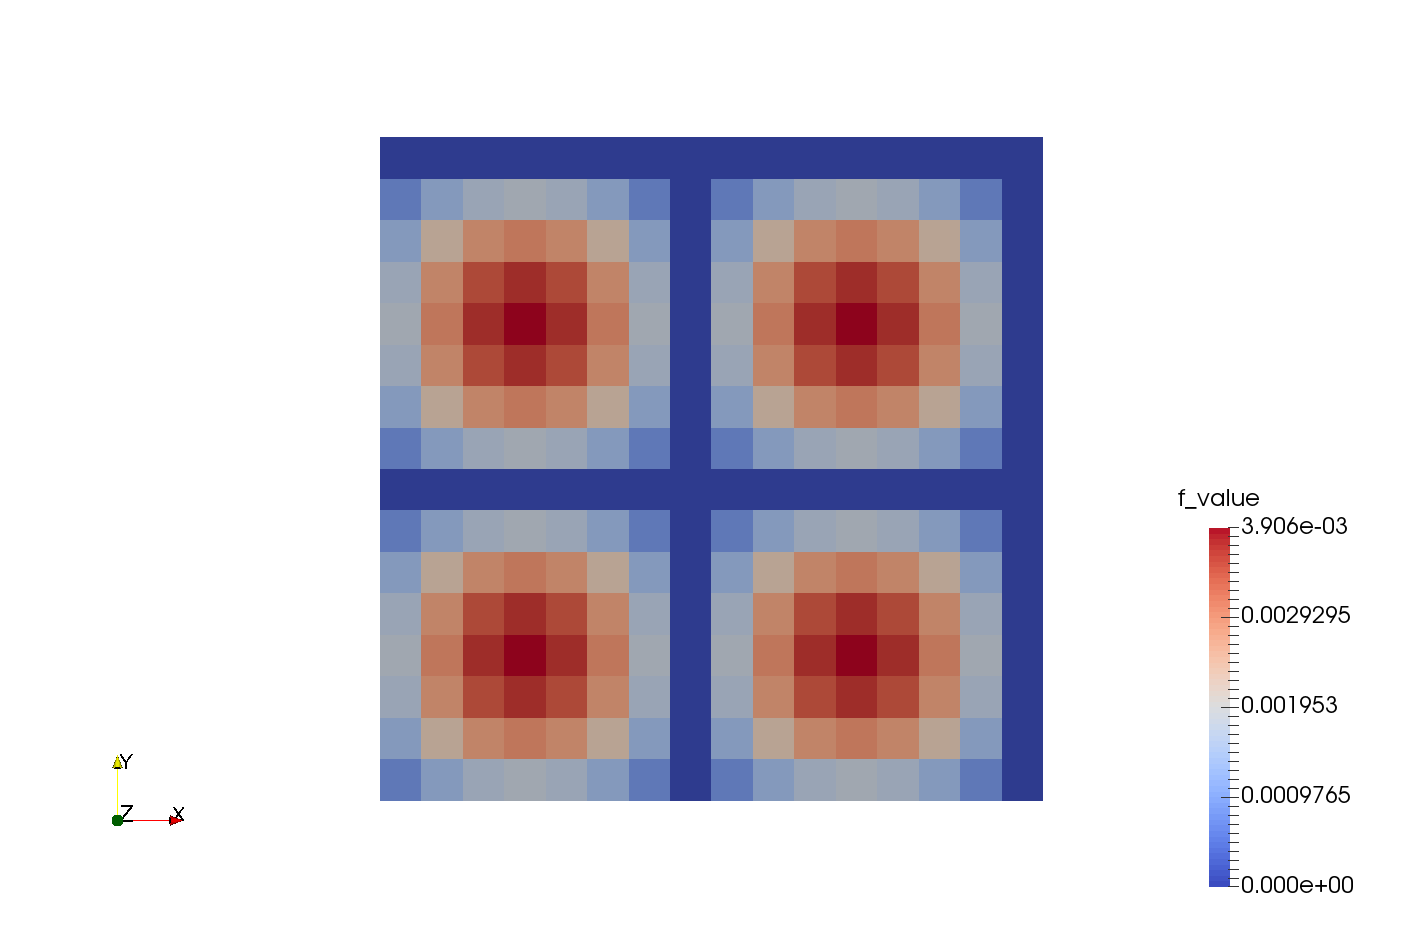
\includegraphics[width =\textwidth]{/results/1/square.png}
		\centering    
	 \caption{}
	 \label{fig:results1Square}
    \end{subfigure} 
    \begin{subfigure}[b]{0.49\textwidth}
	    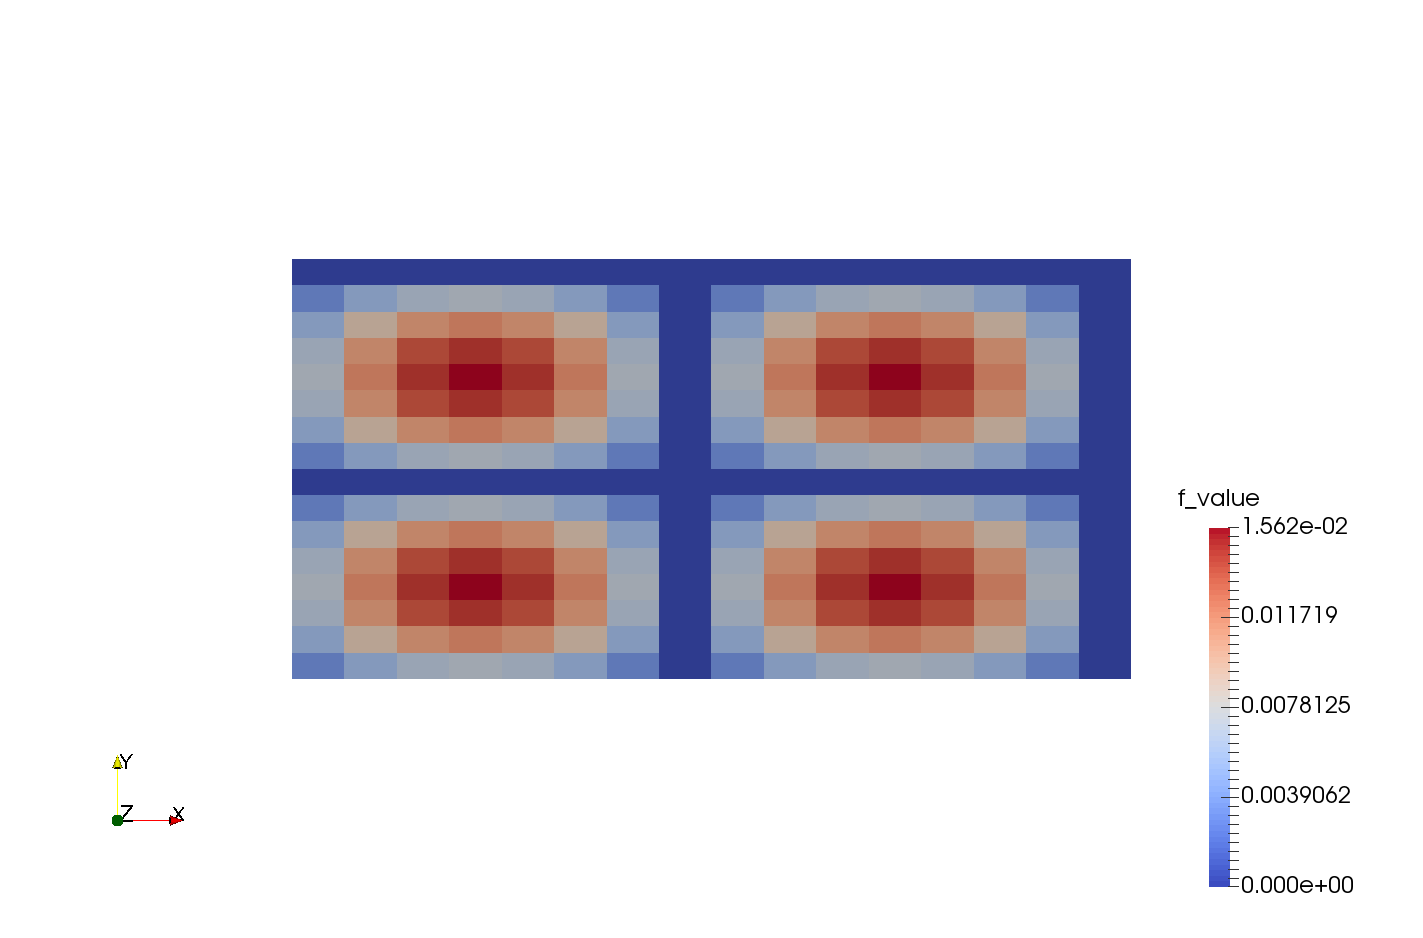
\includegraphics[width =\textwidth]{/results/1/rectangle.png}
	    %\vspace{3em}
		\centering
        \caption{}
        \label{fig:results1Rect}
    \end{subfigure}     
    \caption{The linked structure for a general tree: (a) the node structure; (b) the portion of the data structure associated with a node and its children.}
    \label{fig:results1SquareRect}
\end{figure}

\section{Verification of components}
In any case, as for any scientific approach, we first need to verify that our implementation works as expected. This has been done by comparison of the solution to normal full grid problem. We present here different test cases to ensure the functionality under a variety of cases.
\begin{enumerate}
\item $f(x)=x^2+y^2$
\item $f(x)=x^2 \cdot y^2 $
\item $f(x)=\sqrt[2]{x} \cdot \sqrt[2]{y}$
\item $f(x)=16 \cdot x(1-x)y(1-y)$
\end{enumerate}
In each case we try to compare the error of combination technique, given the default scheme of $\overrightarrow{l}=(4,4)$.\\

In every case, the figures showing the difference are compiled in figure \ref{fig:results2case1-4Diff} to better observe and compare the extent of the spread of error in the domain. For special test case 1, the results are shown in figure \ref{fig:results2case1}. Since the bilinear interpolation is used in this case, figure shows that the combination technique gives the perfect solution. The reason for this is the nature of problem. Since bilinear interpolation is performed in one direction first and then in the other direction, it can be observe that interpolation of a function which is not of terms $x^even \cdot y^even$ gives no error. Figures \ref{fig:results2case2}-\ref{fig:results2case4} show the results for cases 2-4
%2figure case 1 verification difference, combigrid, fullgrid alll together
\begin{figure}[h]
	\centering
    \begin{subfigure}[b]{0.49\textwidth}
	    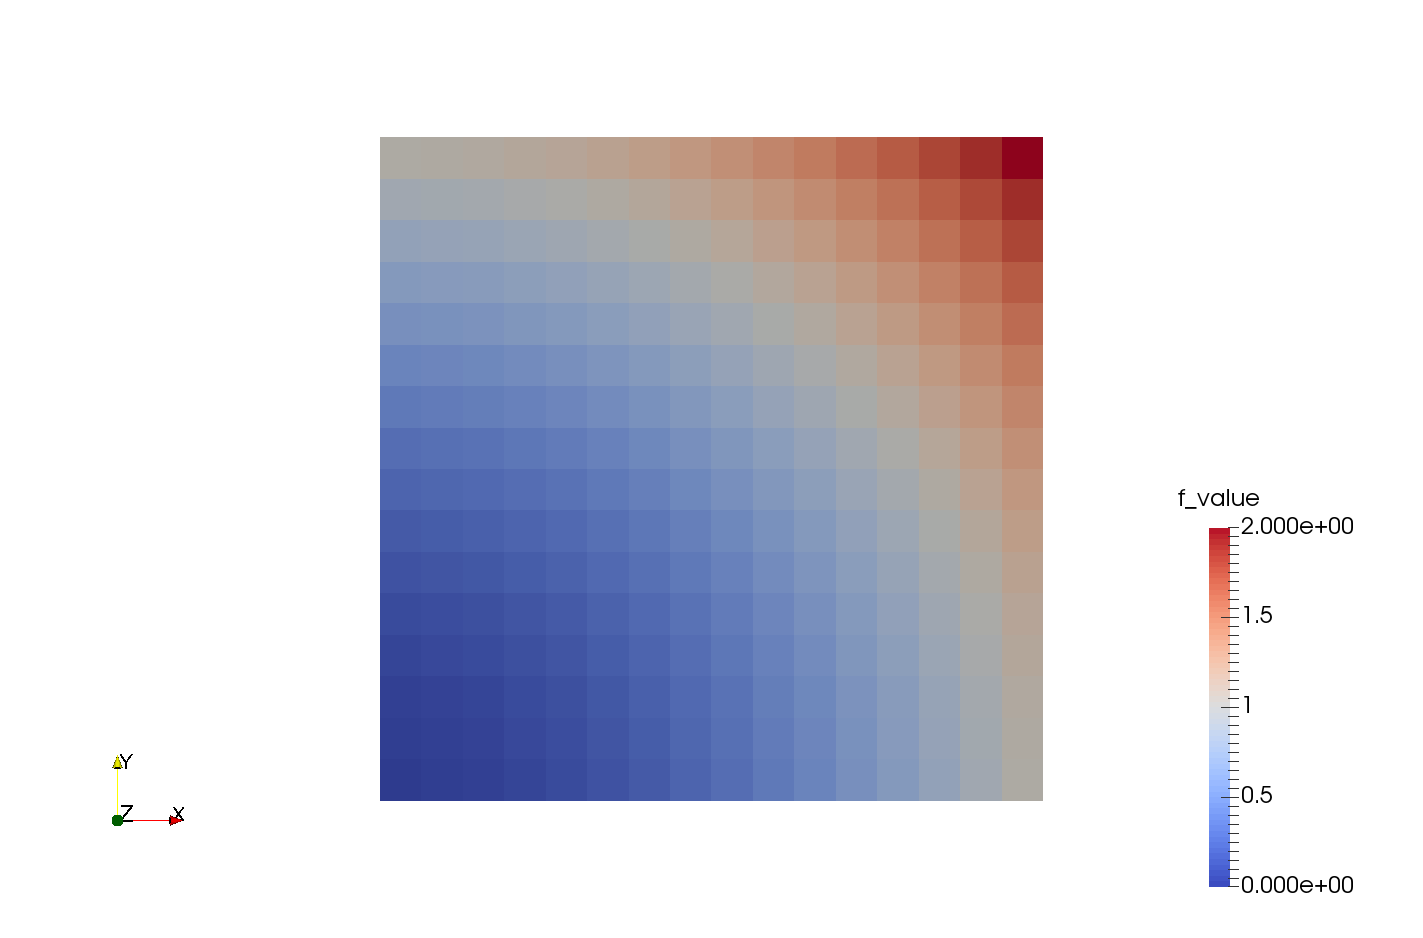
\includegraphics[width =\textwidth]{/results/2/case1-verification-combination.png}
	    %\vspace{3em}
		\centering
        \caption{Combination}
        \label{fig:results2case1Combi}
    \end{subfigure} 
    \begin{subfigure}[b]{0.49\textwidth}    
	    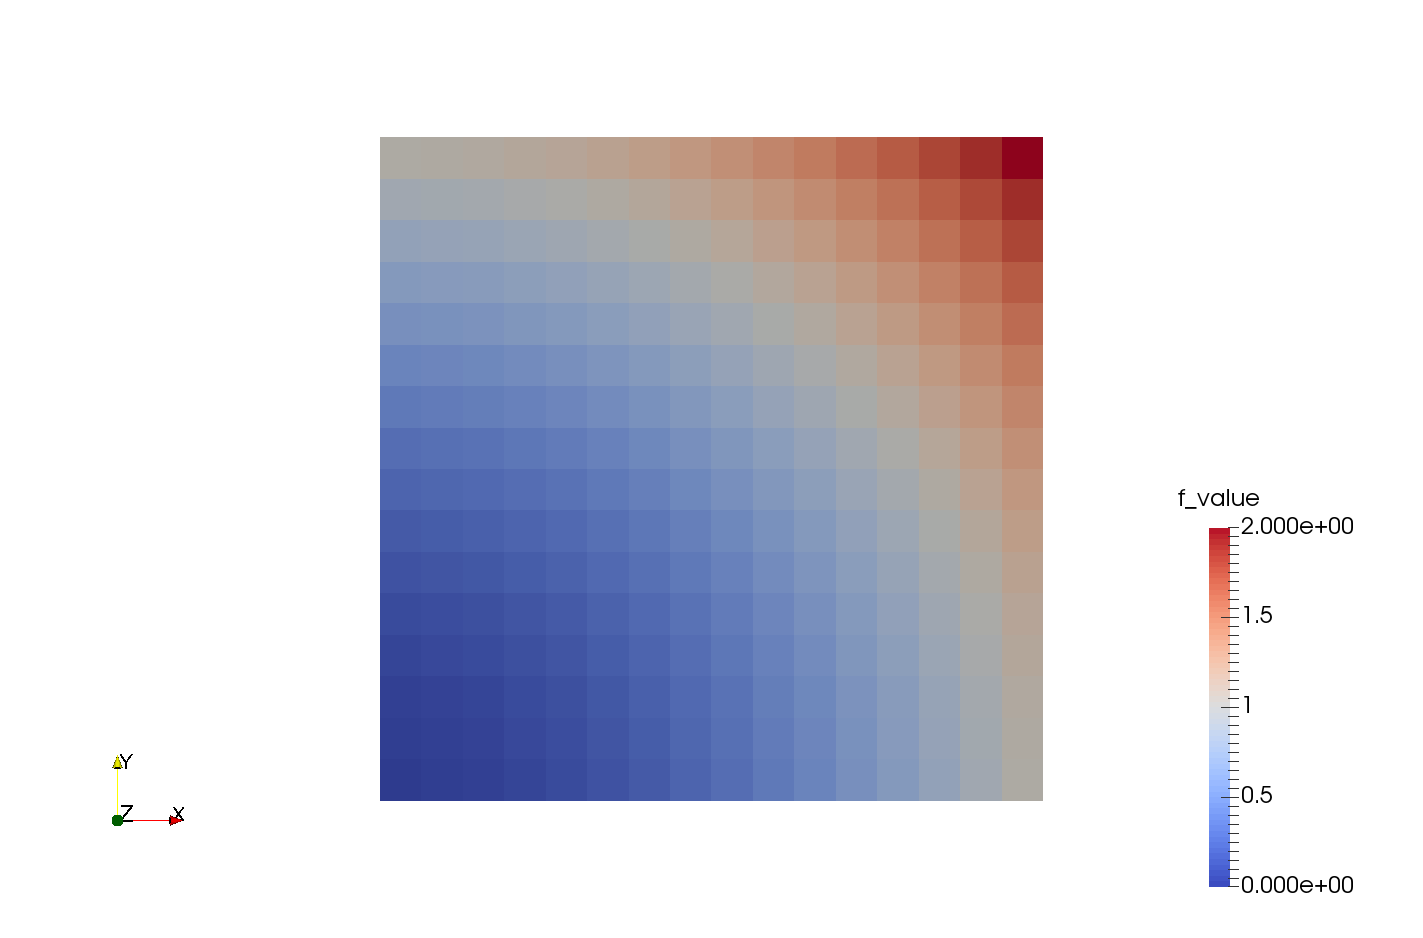
\includegraphics[width =\textwidth]{/results/2/case1-verification-fullgrid.png}
		\centering    
		 \caption{Verification}
	    \label{fig:results2case1Full}	 
    \end{subfigure} 
    \caption{(a) Combination and (b) verification for case 1}
    \label{fig:results2case1}
\end{figure}
%2figure case 2 verification difference, combigrid, fullgrid alll together
\begin{figure}[h]
	\centering
    \begin{subfigure}[b]{0.49\textwidth}
	    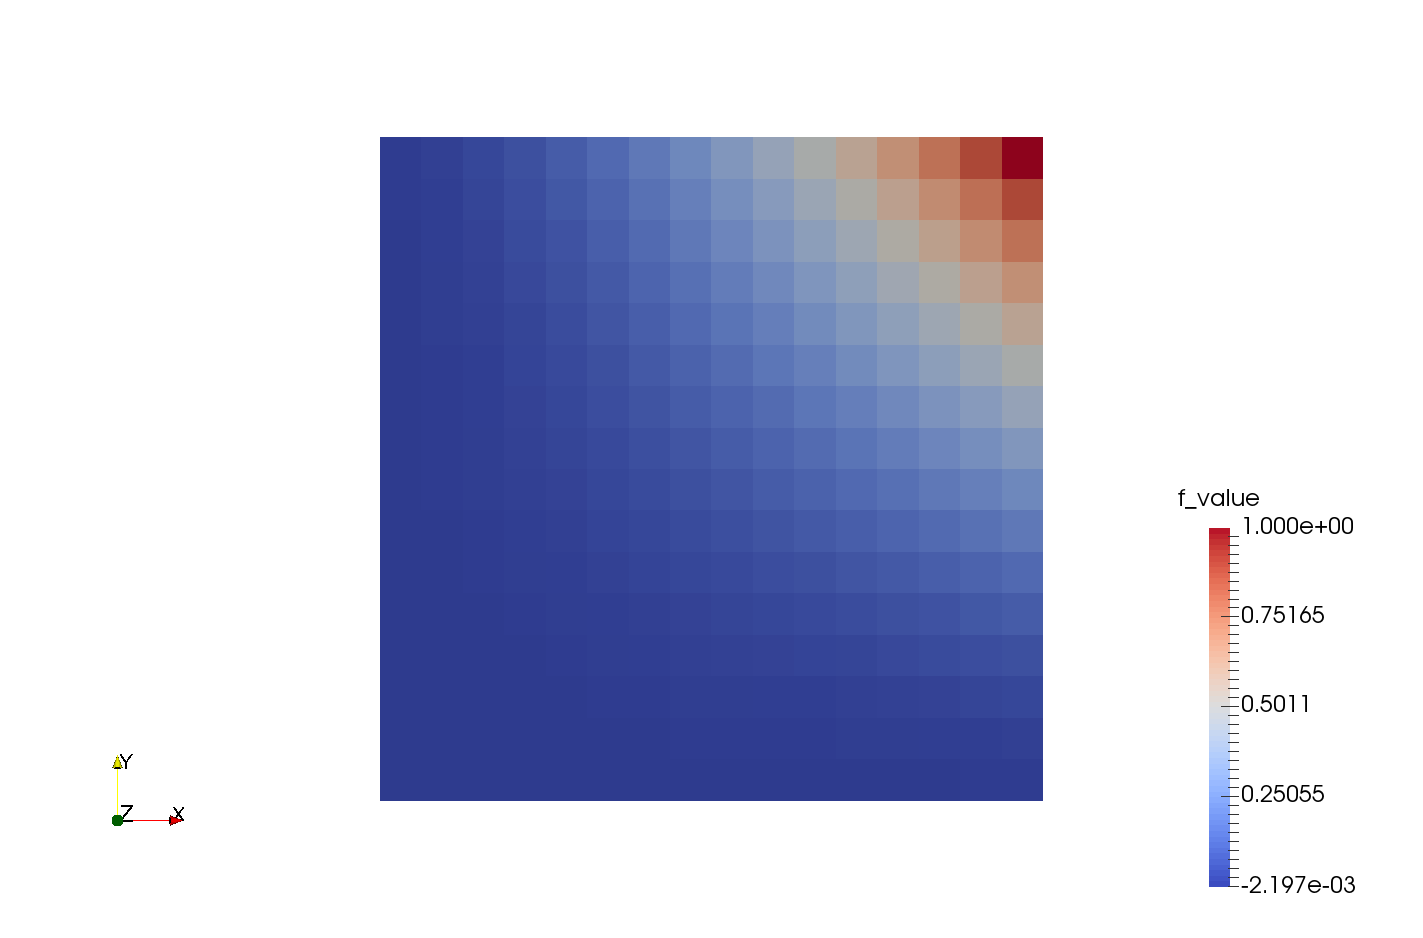
\includegraphics[width =\textwidth]{/results/2/case2-verification-combination.png}
	    %\vspace{3em}
		\centering
        \label{fig:results2case2Combi}
        \caption{Combination}
    \end{subfigure} 
    \begin{subfigure}[b]{0.49\textwidth}    
	    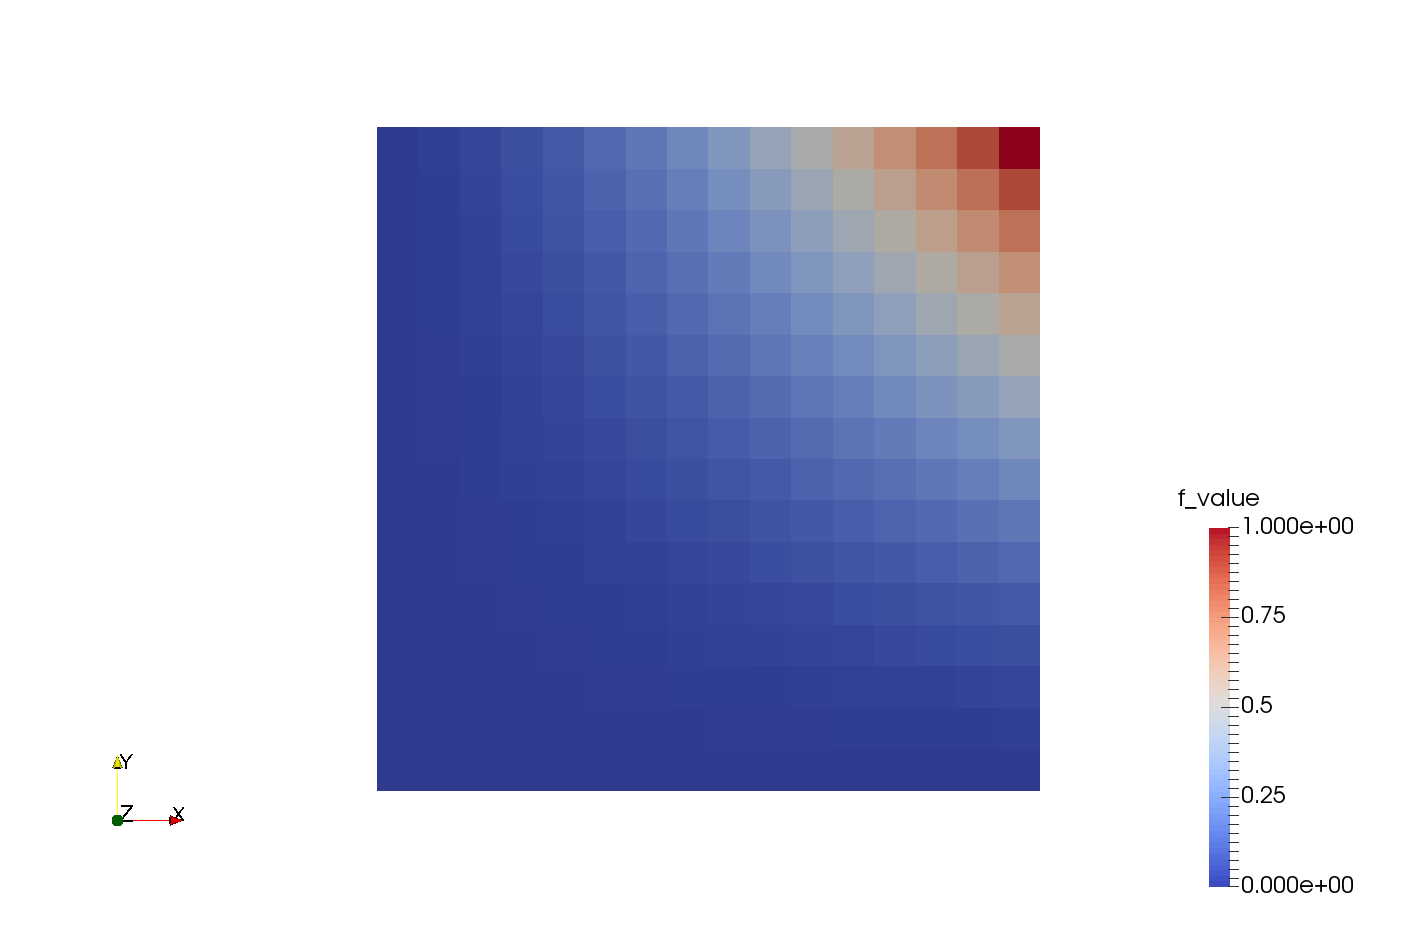
\includegraphics[width =\textwidth]{/results/2/case2-verification-fullgrid.png}
		\centering    
	 \caption{Verification}
	    \label{fig:results2case2Full}	 	 
    \end{subfigure} 
    \caption{(a) Combination and (b) verification for case 2}
    \label{fig:results2case2}
\end{figure}
%2figure case 3 verification difference, combigrid, fullgrid alll together
\begin{figure}[h]
	\centering
    \begin{subfigure}[b]{0.49\textwidth}
	    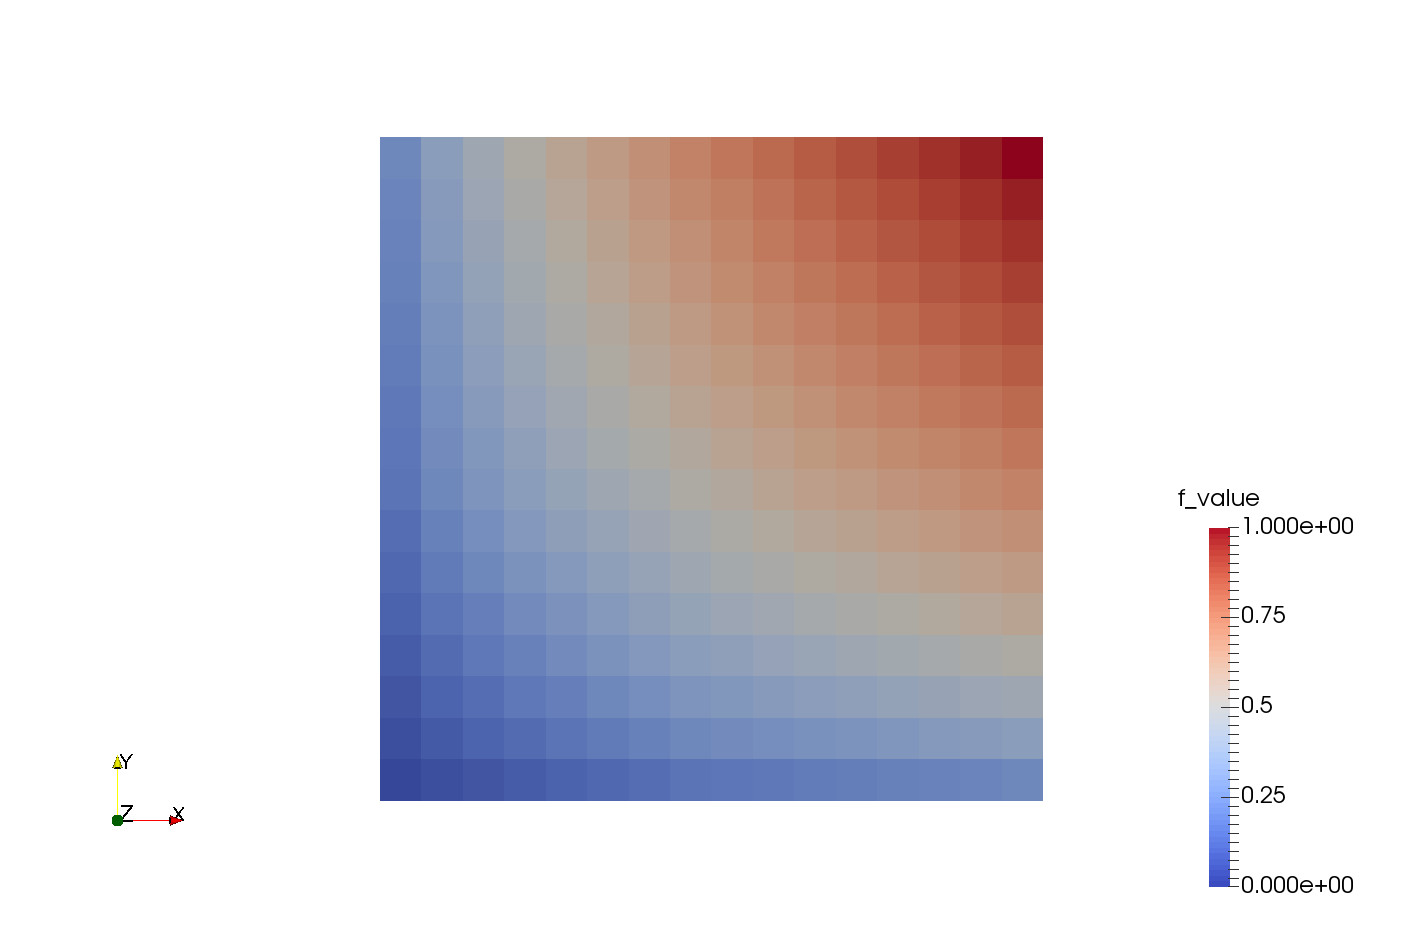
\includegraphics[width =\textwidth]{/results/2/case3-verification-combination.png}
	    %\vspace{3em}
		\centering
        \label{fig:results2case3Combi}
        \caption{Combination}
    \end{subfigure} 
    \begin{subfigure}[b]{0.49\textwidth}    
	    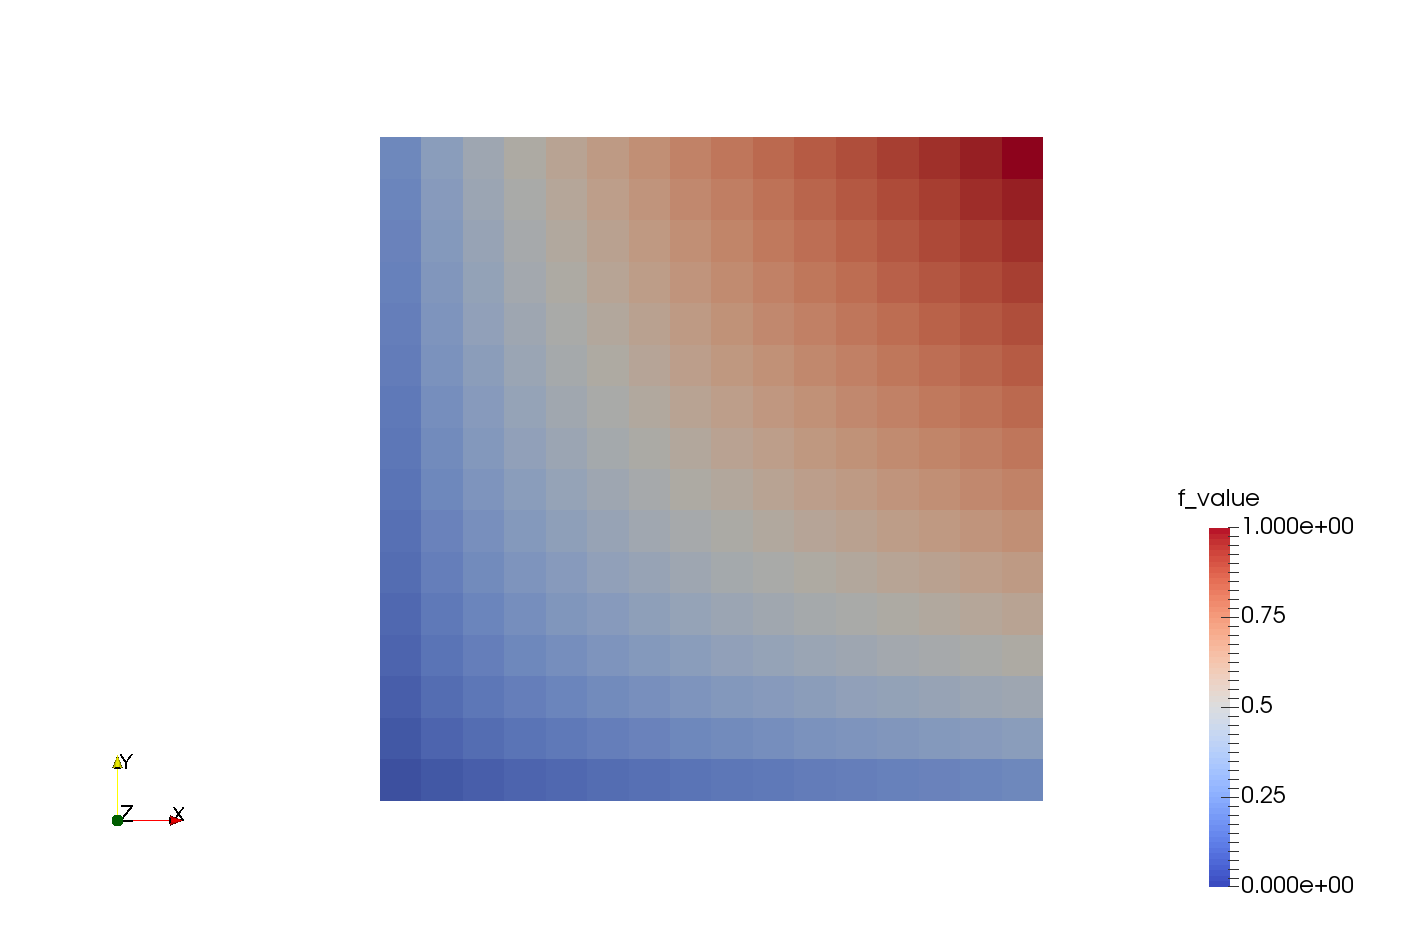
\includegraphics[width =\textwidth]{/results/2/case3-verification-fullgrid.png}
		\centering    
	 \caption{Verification}
	    \label{fig:results2case3Full}	 	 
    \end{subfigure} 
    \caption{(a) Combination and (b) verification for case 3}
    \label{fig:results2case3}
\end{figure}
%2figure case 4 verification difference, combigrid, fullgrid alll together
\begin{figure}[h!]
	\centering
    \begin{subfigure}[b]{0.49\textwidth}
	    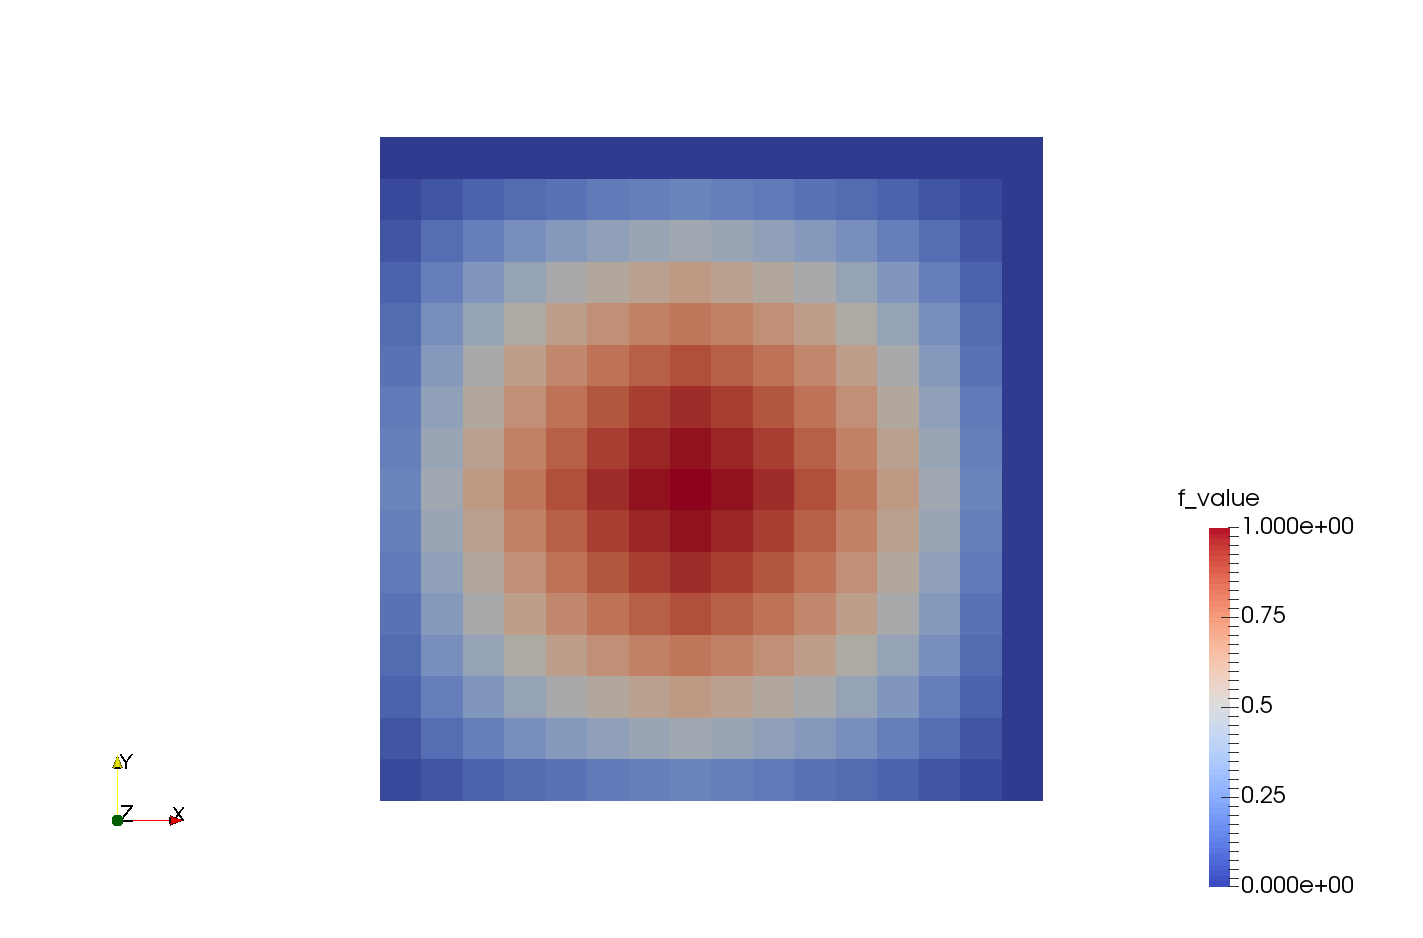
\includegraphics[width =\textwidth]{/results/2/case4-verification-combination.png}
	    %\vspace{3em}
		\centering
        \label{fig:results2case4Combi}
        \caption{Combination}
    \end{subfigure} 
    \begin{subfigure}[b]{0.49\textwidth}    
	    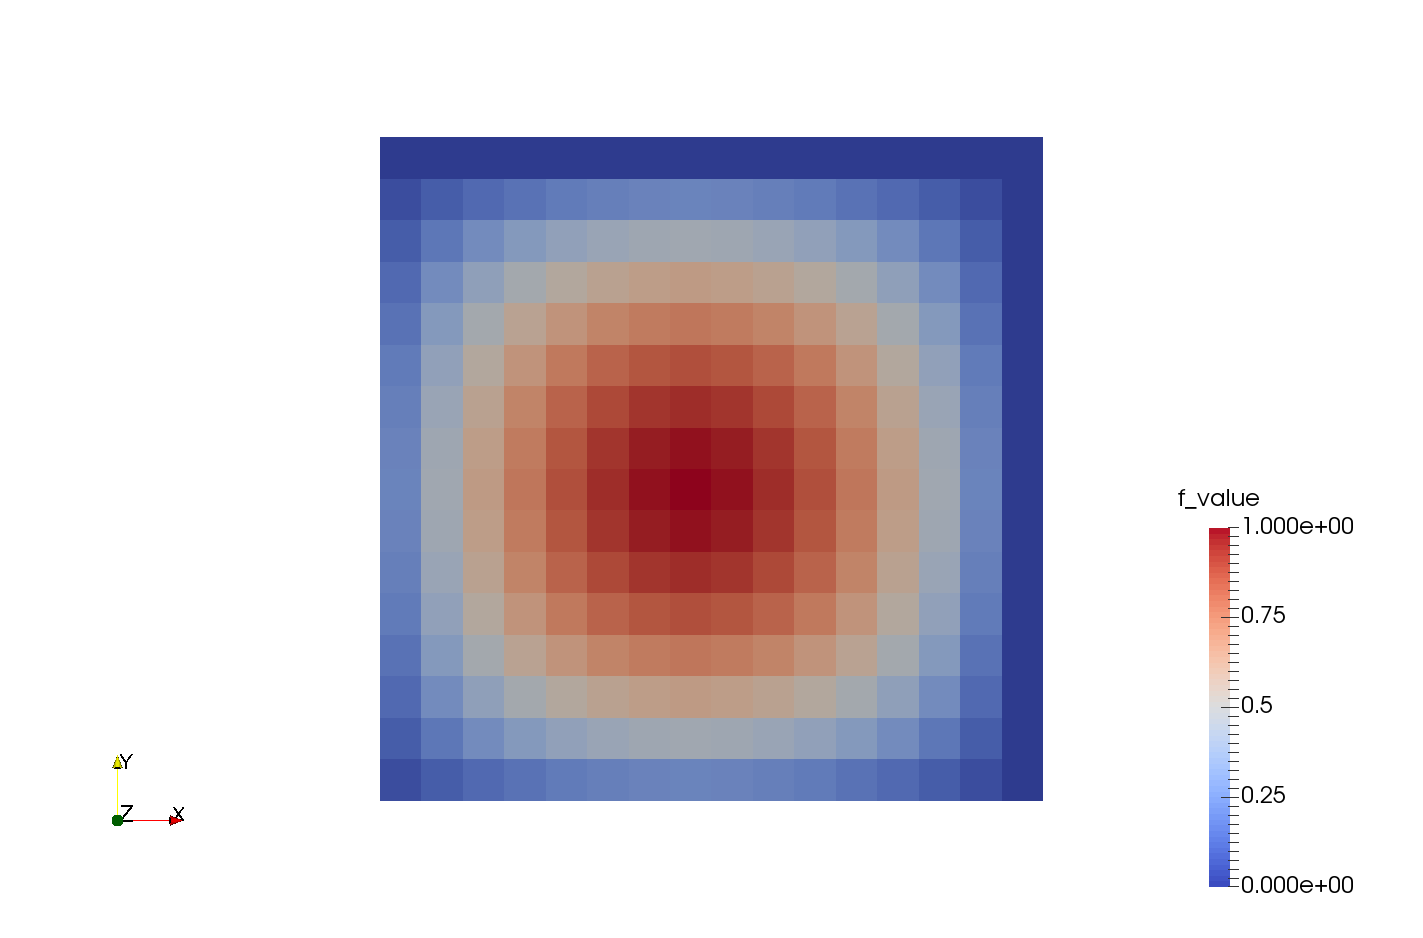
\includegraphics[width =\textwidth]{/results/2/case4-verification-fullgrid.png}
		\centering    
	 \caption{Verification}
	    \label{fig:results2case4Full}	 	 
    \end{subfigure} 
    \caption{(a) Combination and (b) verification for case 4}
    \label{fig:results2case4}
\end{figure}

%Case 1-4 differences
\begin{figure}[h!]
	\centering
    \begin{subfigure}[b]{0.49\textwidth}
	    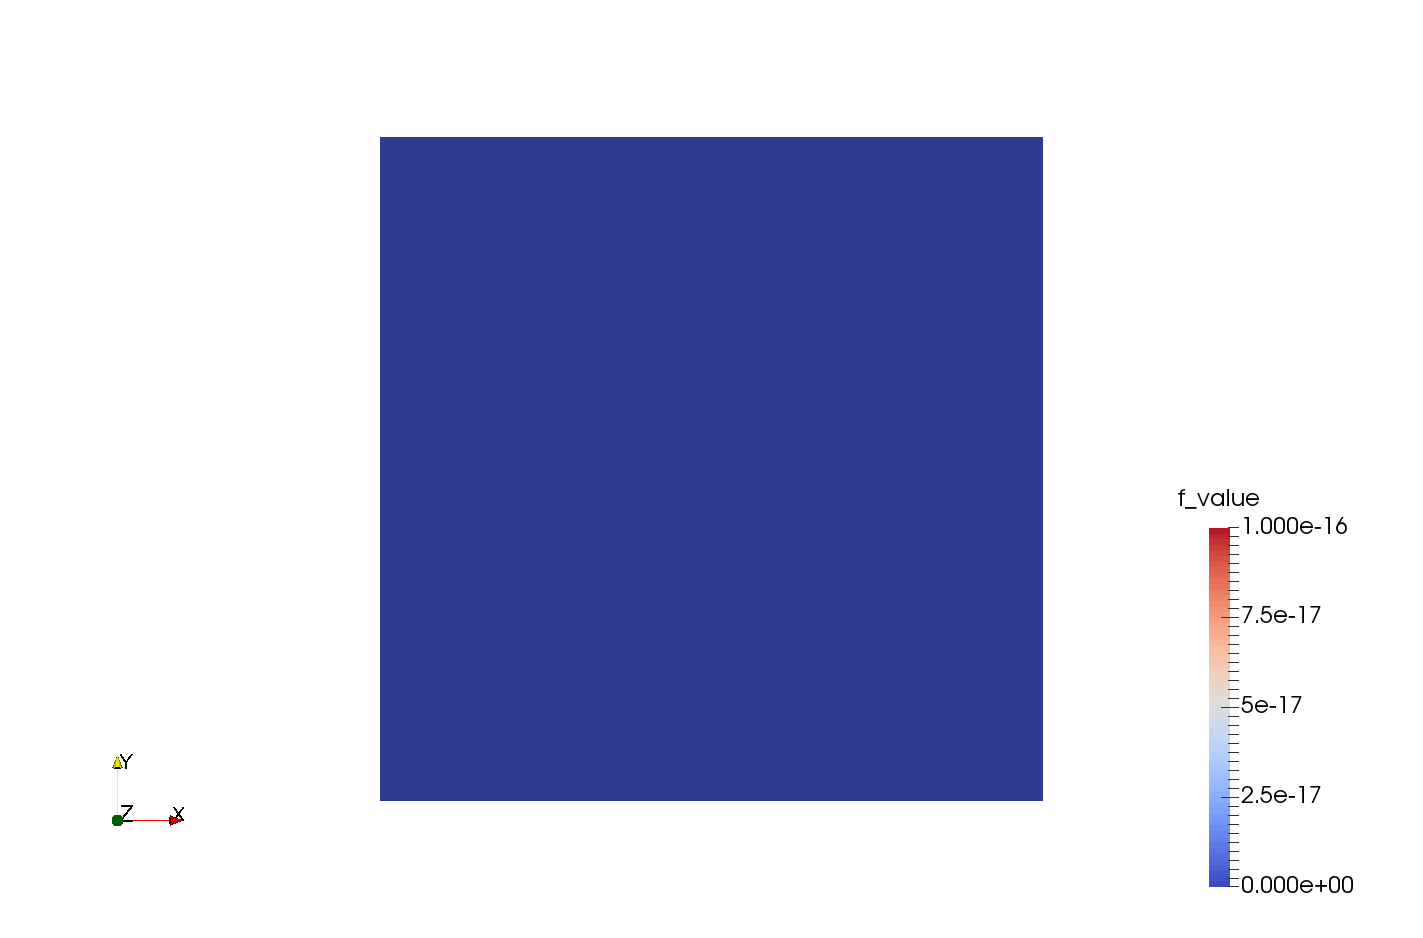
\includegraphics[width =\textwidth]{/results/2/case1-verification-difference.png}
	    %\vspace{3em}
		\centering
        \label{fig:results2case1Diff}
        \caption{Case 1}
    \end{subfigure} 
    \begin{subfigure}[b]{0.49\textwidth}    
	    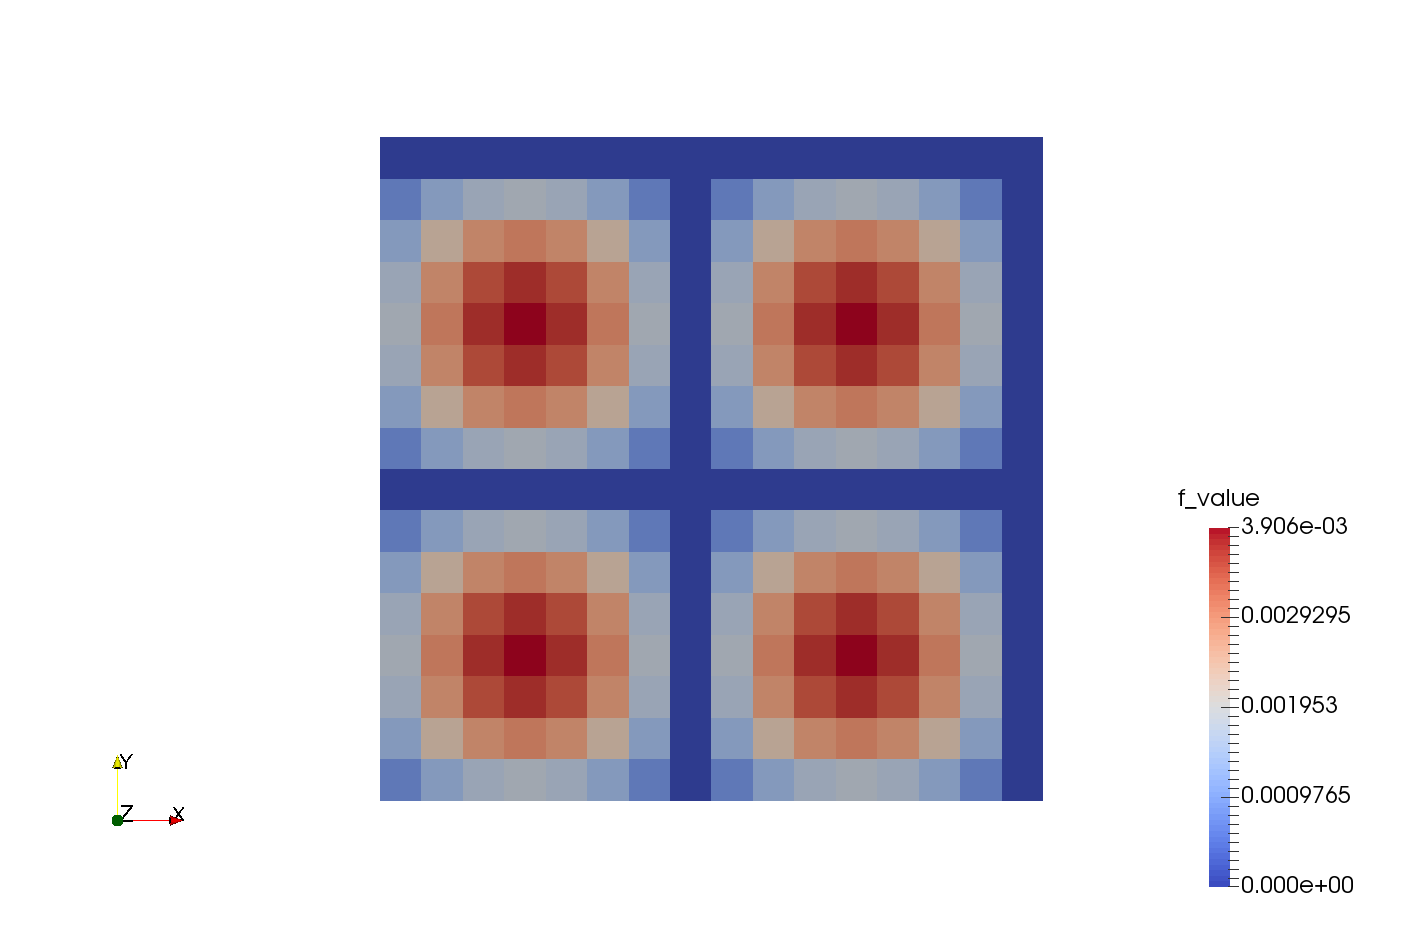
\includegraphics[width =\textwidth]{/results/2/case2-verification-difference.png}
		\centering    
	 \caption{Case 2}
	    \label{fig:results2case2Diff}	 	 
    \end{subfigure} 
    \begin{subfigure}[b]{0.49\textwidth}
	    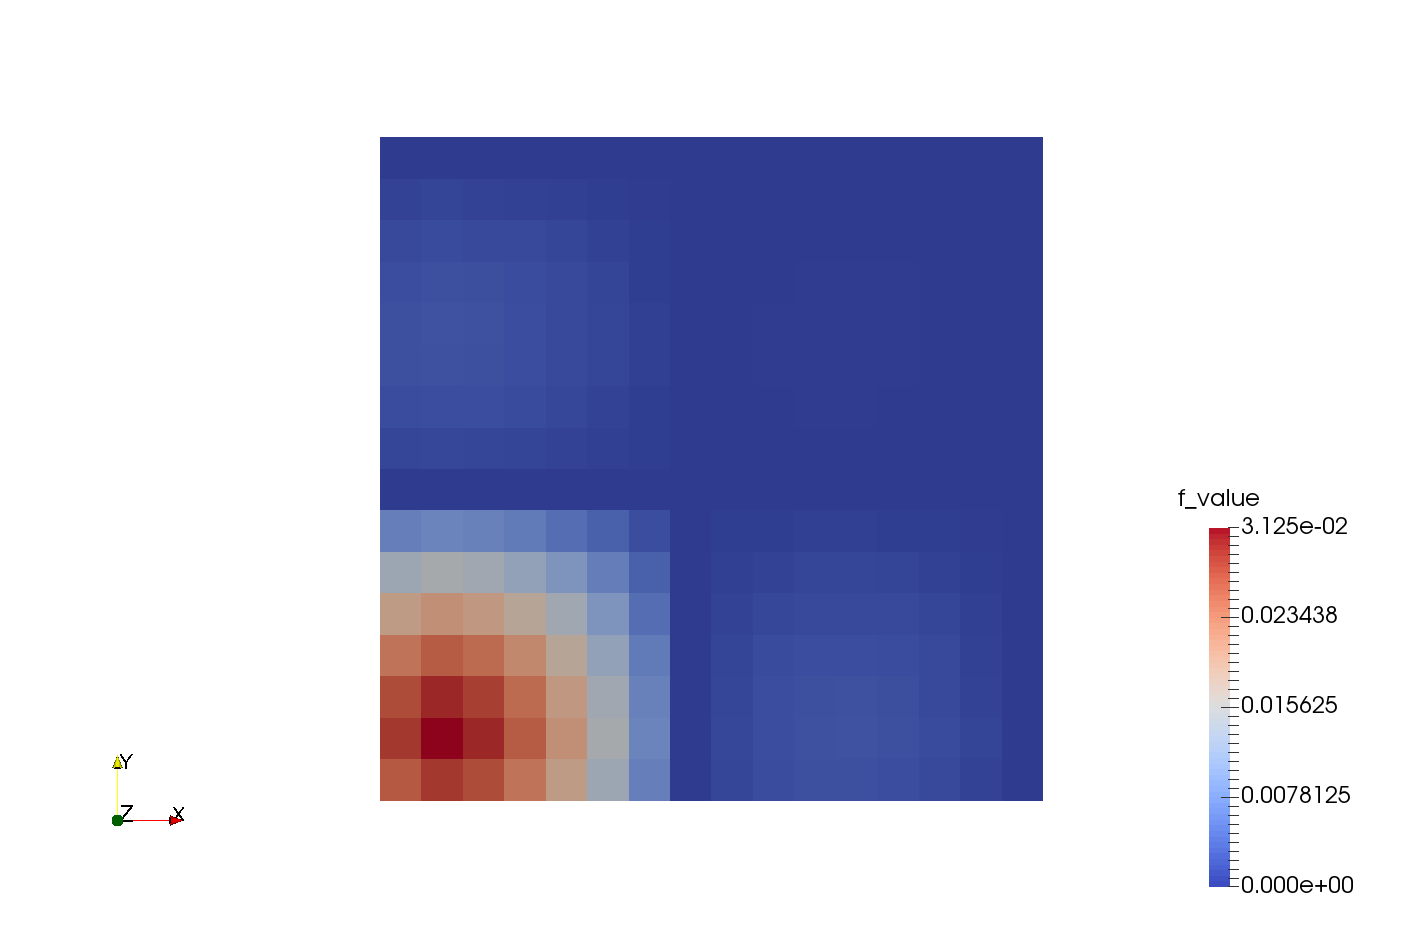
\includegraphics[width =\textwidth]{/results/2/case3-verification-difference.png}
	    %\vspace{3em}
		\centering
        \label{fig:results2case3Diff}
        \caption{Case 3}
    \end{subfigure} 
    \begin{subfigure}[b]{0.49\textwidth}    
	    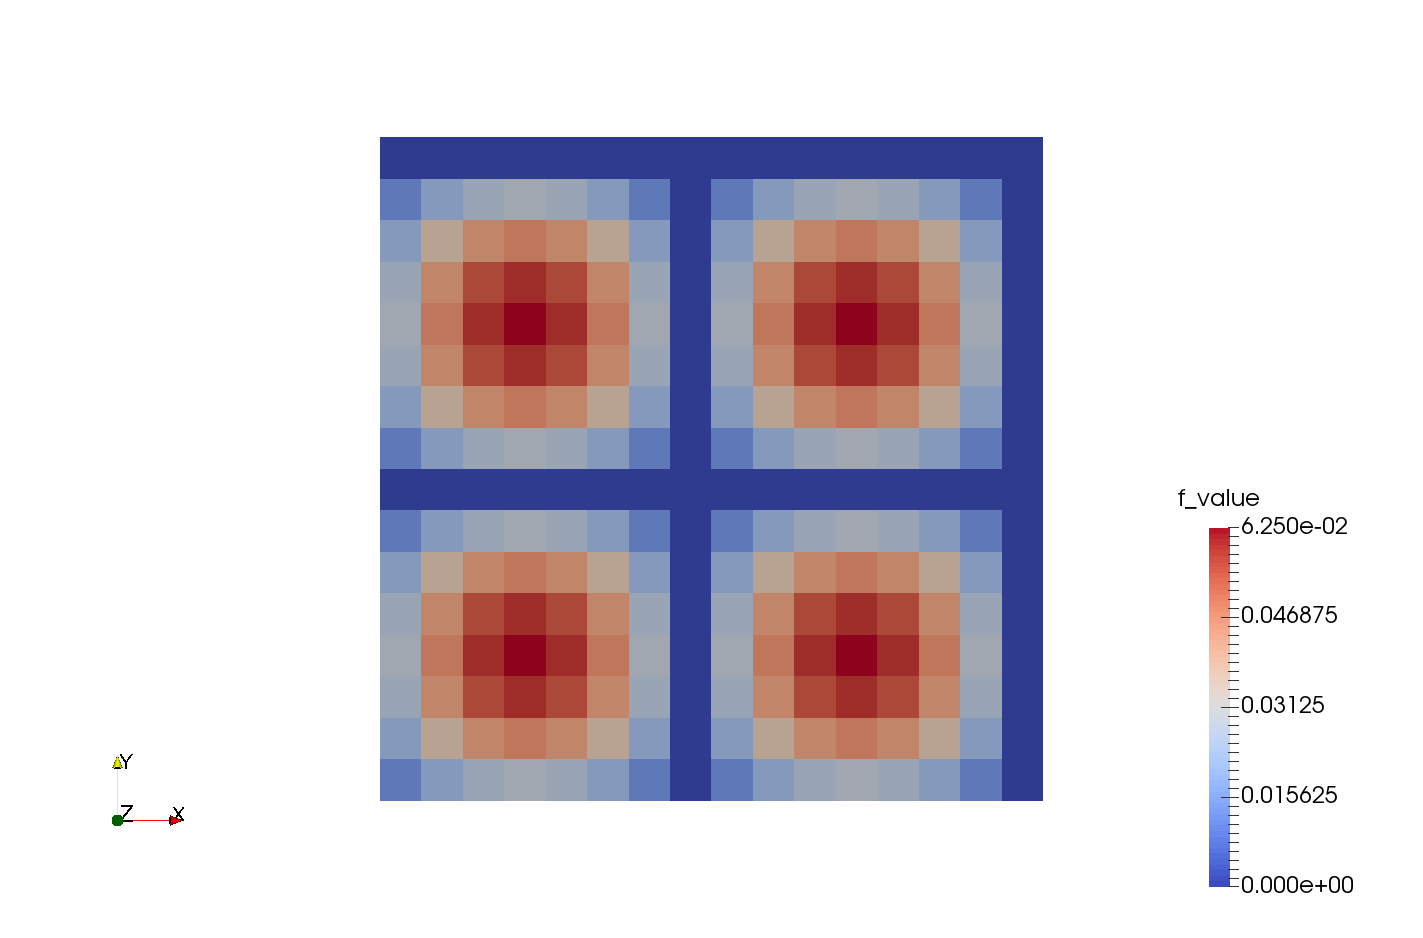
\includegraphics[width =\textwidth]{/results/2/case4-verification-difference.png}
		\centering    
	 \caption{Case 4}
	    \label{fig:results2case4Diff}	 	 
    \end{subfigure} 
    \caption{Difference case 1-4}
    \label{fig:results2case1-4Diff}
\end{figure}


The absolute values of the general error for cases 1 to 4 are compiled in the table \ref{table:GenError}. The general error is 0 for case 1, as already discussed. Case 4 shows a much higher absolute error as the function has a multiplicative factor of 16, leading to higher function values. 

\begin{table}[h]
\centering
\label{table:GenError}
\caption{The resulting general error for cases 1-4 for verification of components}
\vspace{1em}
\begin{tabular}{| c | c | c |}
\hline
 Test Case Number & Function &  General Error\\
 \hline
 1 & $f(x)=x^2+y^2$ & 0 \\
 \hline
 2 & $f(x)=x^2 \cdot y^2 $ & 0.4306\\
 \hline
 3 & $f(x)=\sqrt[2]{x} \cdot \sqrt[2]{y}$ & 0.9224\\
 \hline
 4 & $f(x)=16 \cdot x(1-x)y(1-y)$ & 6.8906 \\
 \hline
\end{tabular}
\end{table}

\section{Results of local refinement (spatial adaptivity)}
Based on the the fact that the current method has been verified, next two different cases are checked for local refinement -- one simply to ensure the proper functionality of the implementation of recursive tree,  and second for the test cases presented above. 

\subsection{Error indicator based on predefined error function}
As explained earlier, the objective here is to come up with a valid test case for local refinement. Based on author's background in mesh generation, there is a technique specially for unstructured grid generation with background predefined function \cite{Henshaw1996} and adaptive grid generation algorithm\cite{Ebeida2010}. Motivated by ideas presented we will enforce a predefined error to the problem by defining an error function which is higher than our threshold for certain regions. This way we can predict the expected working of the local refinement exactly. For better clarity, the solution tree structure is presented in figure \ref{fig:QuadTreeRoot} and the predefined function with it's image on the unit square problem is presented in figure \ref{fig:Predef}.\\

% 3figure of tree from aastha
% 3figure of predefined error from aastha

\begin{figure}[h]
	\centering
	    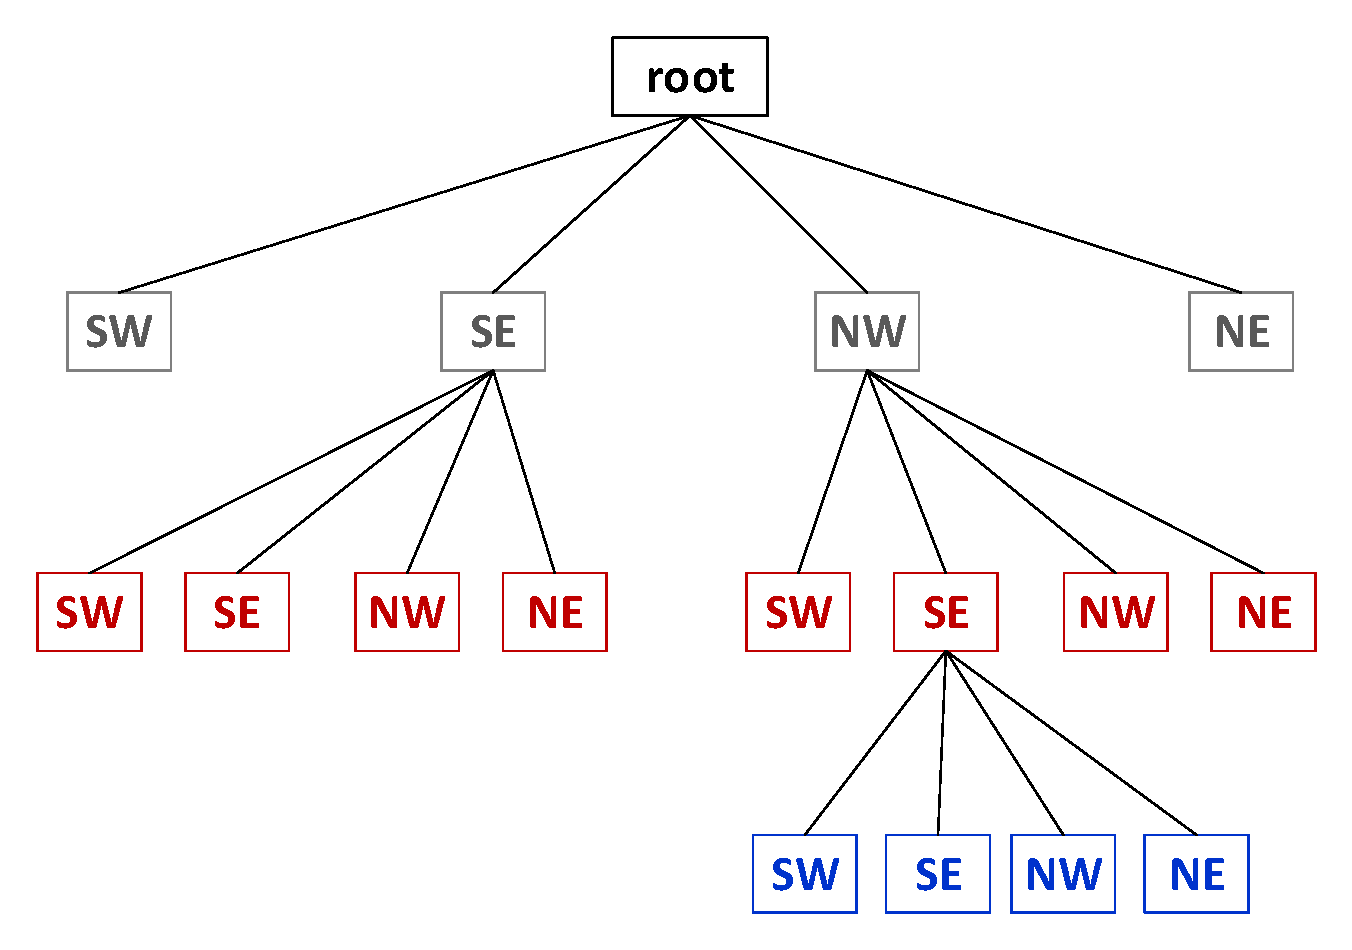
\includegraphics[width =0.66\textwidth]{/results/3/QuadTreeRoot.pdf}
	    %\vspace{3em}
		\centering
        \caption{Quad tree representation}
        \label{fig:QuadTreeRoot}
\end{figure}


		
\begin{figure}[h]
	\centering
    \begin{subfigure}[b]{0.66\textwidth}    
	    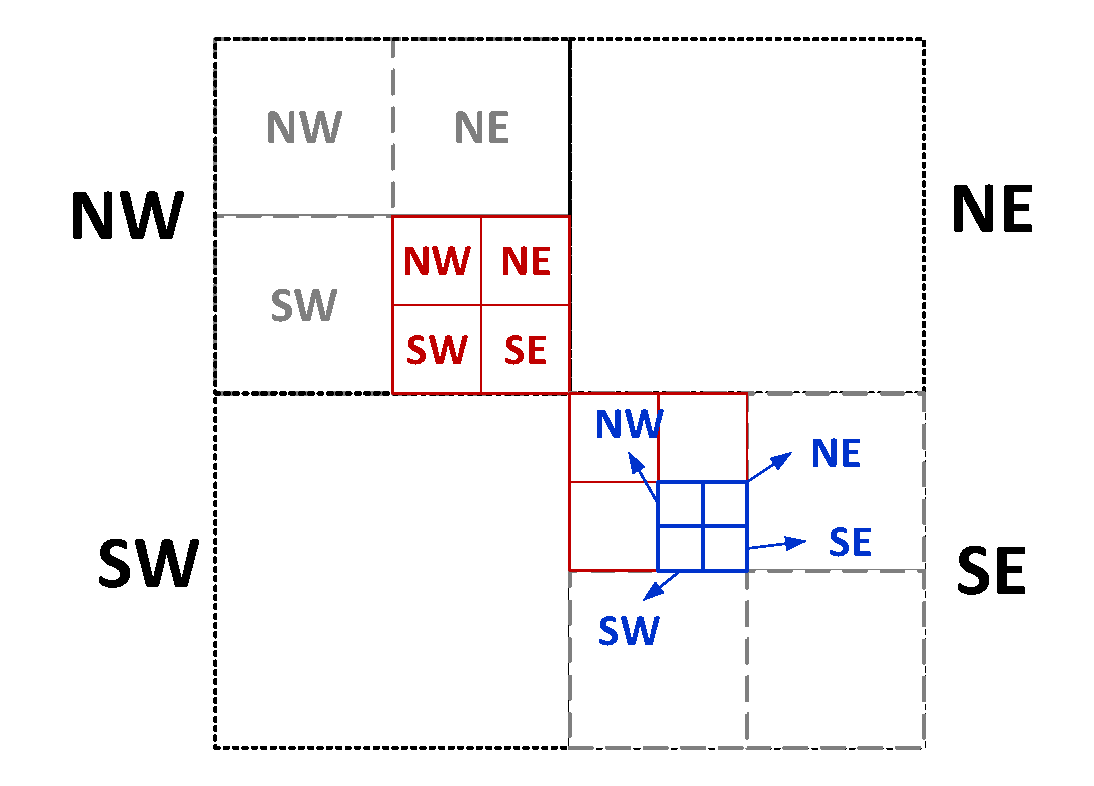
\includegraphics[width =\textwidth]{/results/3/QuadTreeSquare.pdf}
		\centering    
		\caption{Quad tree}
		\label{fig:QuadTreeSquare}
    \end{subfigure} 
    \begin{subfigure}[b]{0.75\textwidth}
	    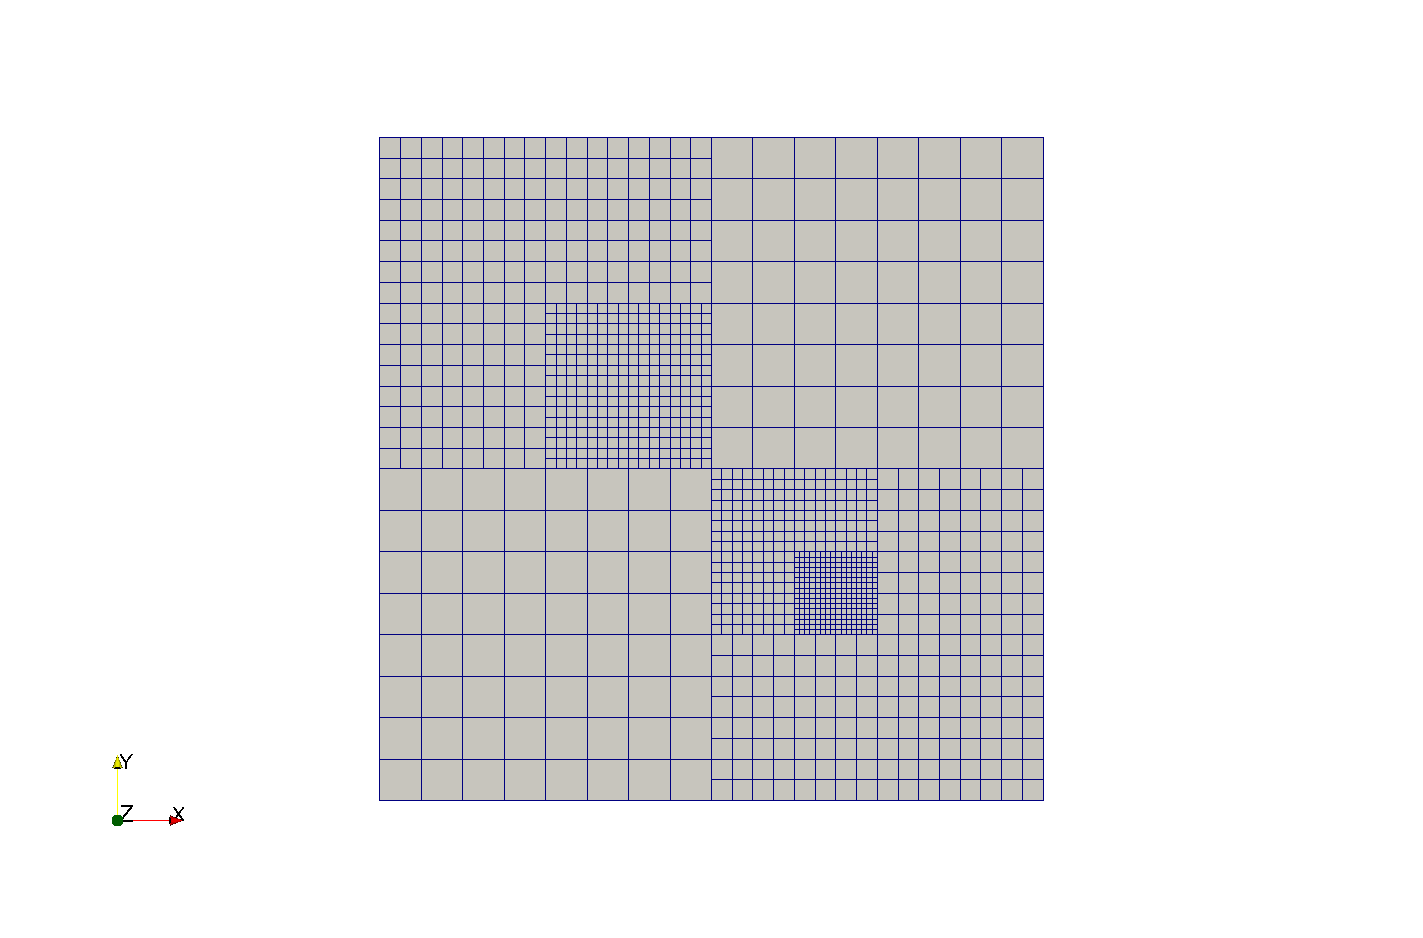
\includegraphics[width =\textwidth]{/results/3/predefined-refinement-vtk.png}
	    %\vspace{3em}
		\centering
        \caption{Predefined refinement}
        \label{fig:PredefRefine}
    \end{subfigure} 
    \caption{Predefined}
    \label{fig:Predef}
\end{figure}

% 3figure predefined refinement from VTK
% 3figure predefined error from VTK

		
\begin{figure}[h]
	\centering
	    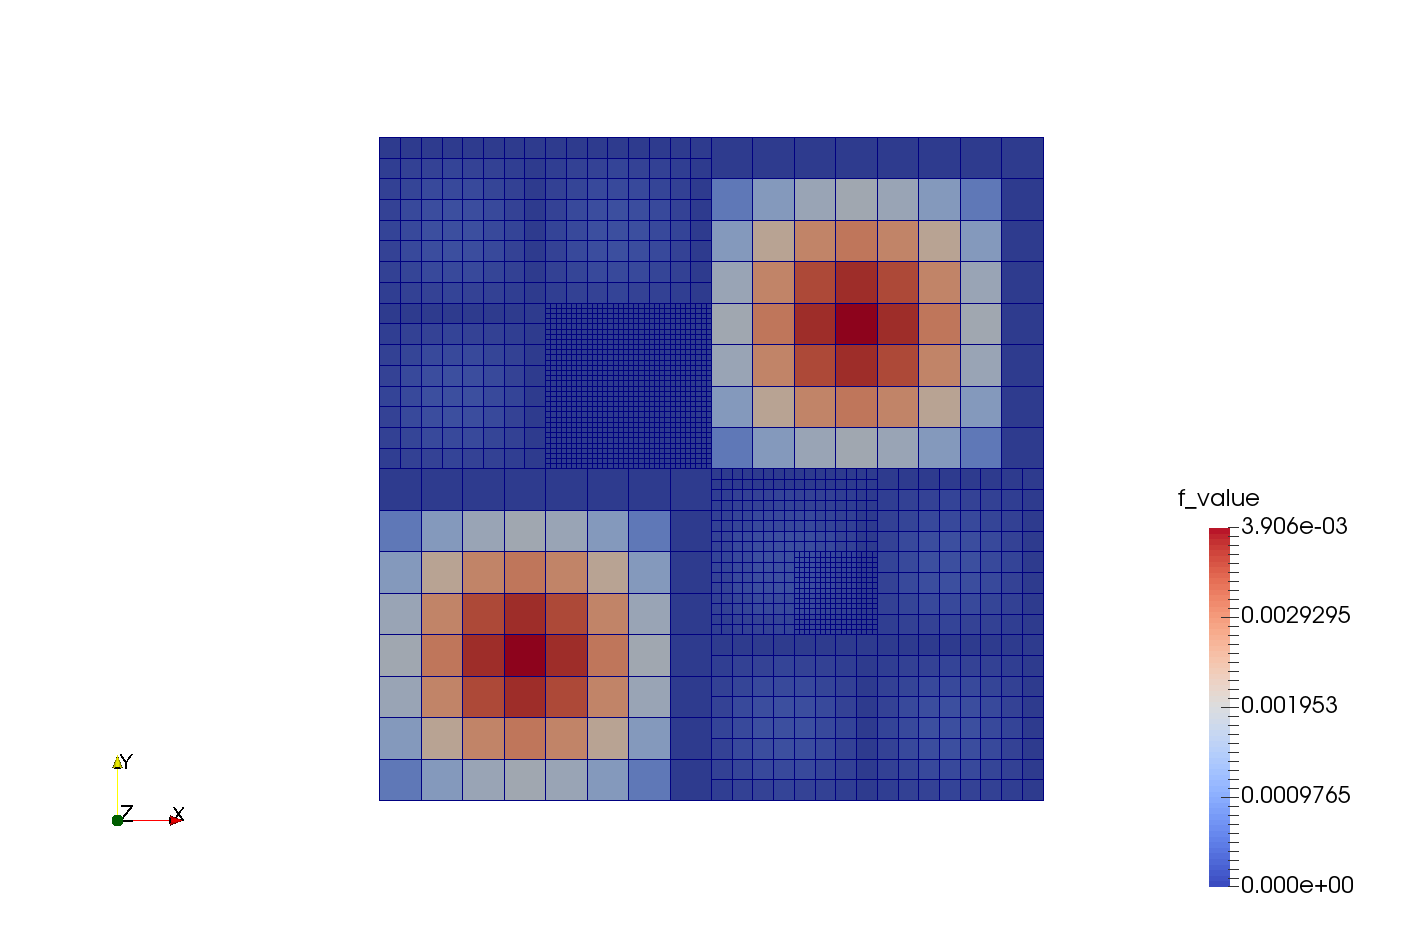
\includegraphics[width =0.75\textwidth]{/results/3/predefined-error-vtk.png}
		\centering    
	 \caption{Predefined error}
       \label{fig:PredefError}
\end{figure}

As seen in figure \ref{fig:PredefError}, the solution to this case matches the expectations. Based on this result, the final evaluation is performed in the next section.

\subsection{Error indicator based on solution of combination technique}
After verification of the code in both adaptive and non-adaptive cases, the next focus is on further investigation into the actual problem at hand, which is performing the adaptation in correspondence with the local error of solution in each node or subtree. For that, an error indicator has been introduced which compares the solution to the full grid method. The primary reason for defining some extra test cases in the verification part was that to be able to observe how the local refinement works with different cases, otherwise there is much similarity between case 2, 3 and 4. The results are visualized in figures \ref{fig:AdaptiveCase2}, \ref{fig:AdaptiveCase3} and \ref{fig:AdaptiveCase4} for cases 2,3 and 4, respectively. \\


%4adaptive case 2: before refinement and after refinement together 
\begin{figure}[h]
	\centering
    \begin{subfigure}[b]{0.49\textwidth}
	    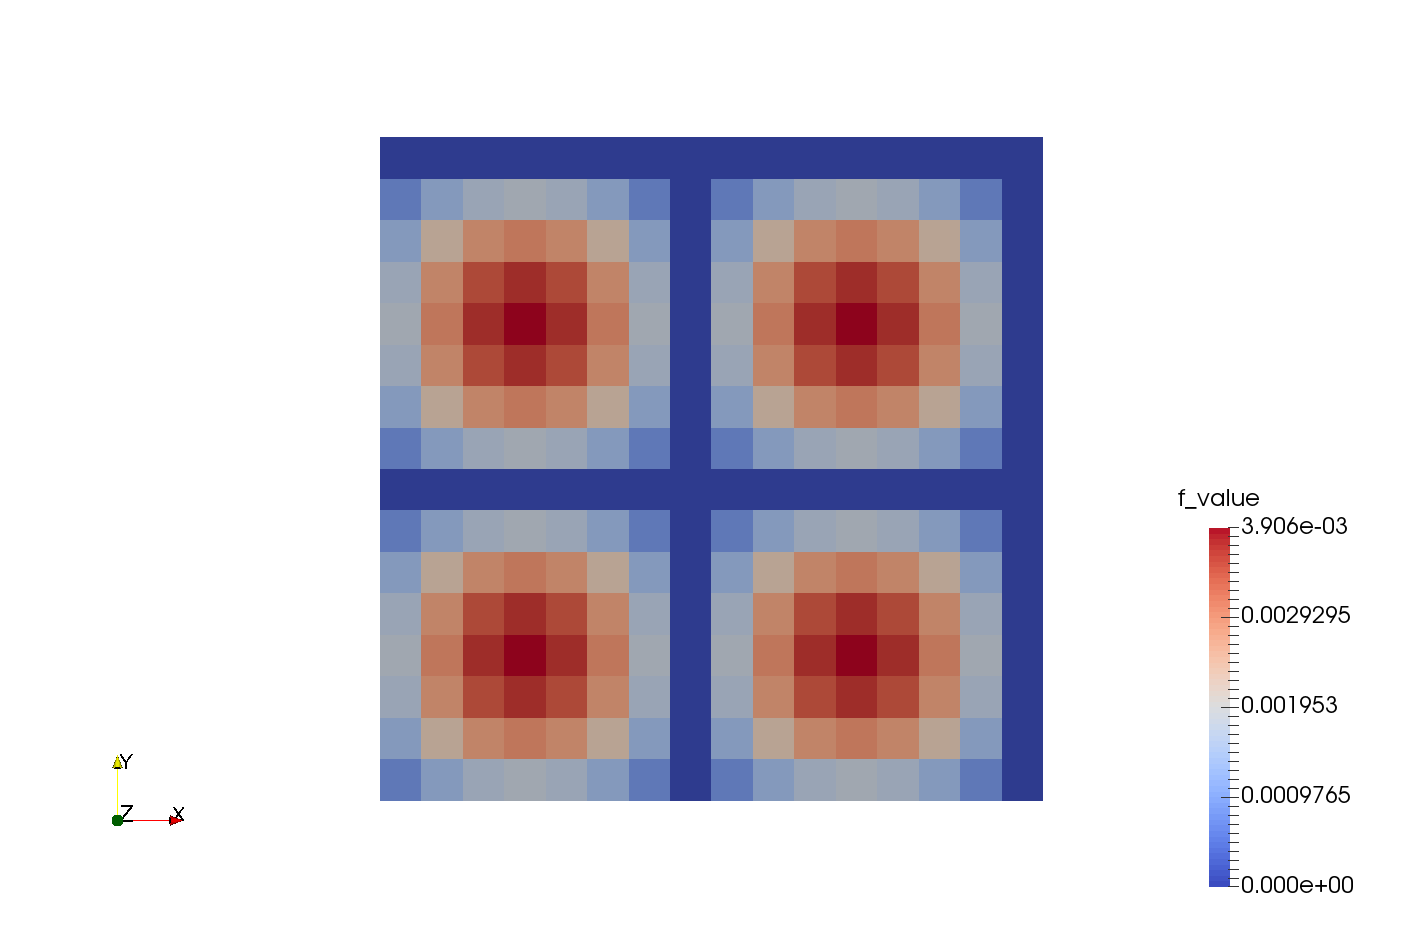
\includegraphics[width =\textwidth]{/results/4/case2-adaptive-before-refinement.png}
	    %\vspace{3em}
		\centering
        \caption{case 2 before refinement}
        \label{fig:AdaptiveCase2Before}
    \end{subfigure} 
    \begin{subfigure}[b]{0.49\textwidth}    
	    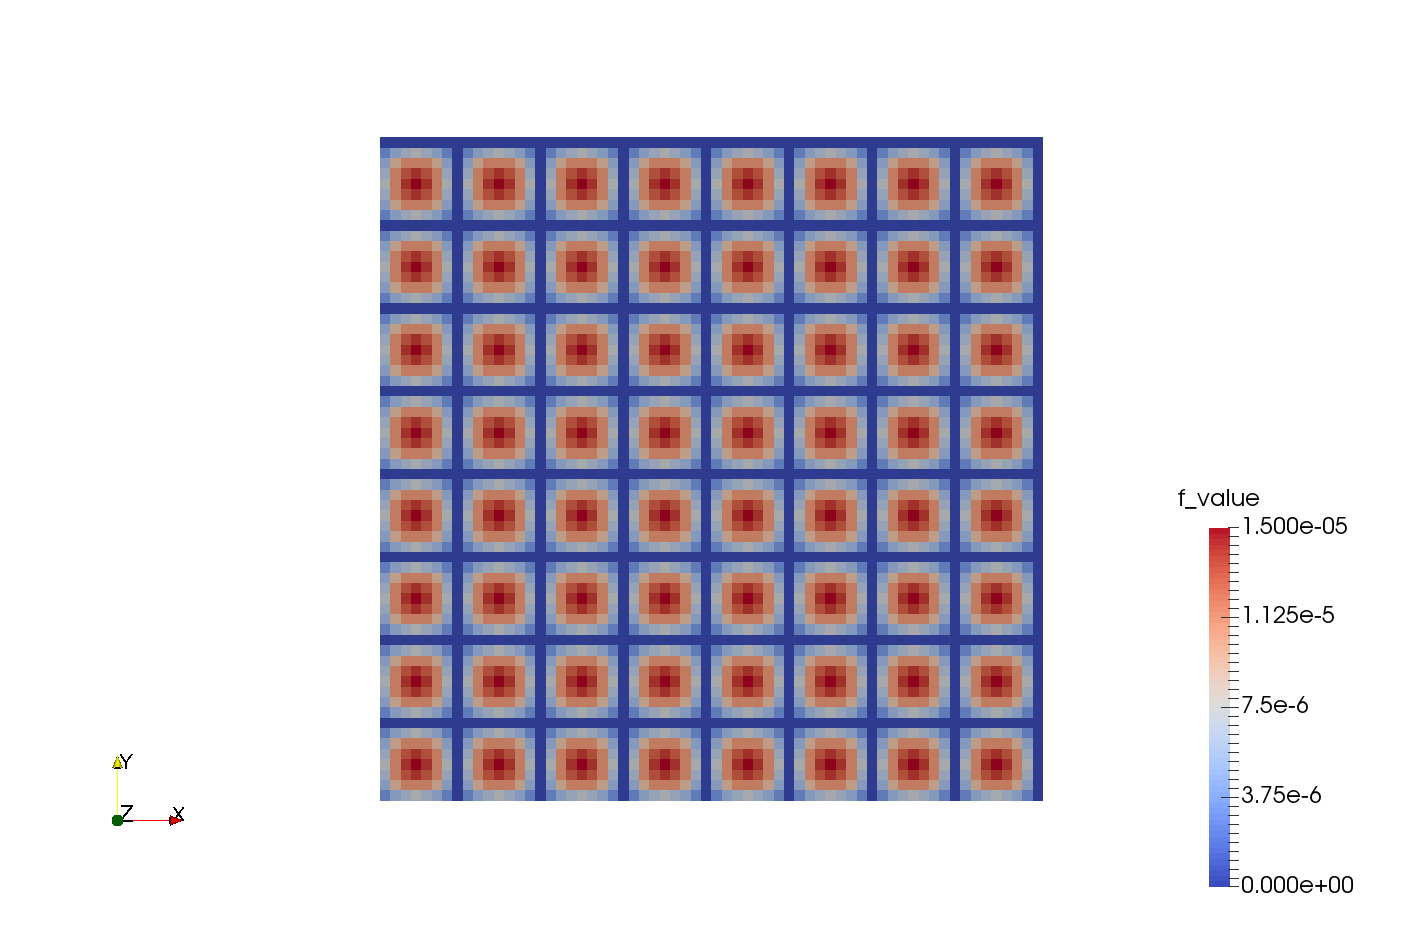
\includegraphics[width =\textwidth]{/results/4/case2-adaptive-after-refinement.png}
		\centering    
	 \caption{case 2 after refinement}
       \label{fig:AdaptiveCase2After}
    \end{subfigure} 
    \caption{Case 2 before and after refinement}
    \label{fig:AdaptiveCase2}
\end{figure}

%4adaptive case 3: before refinement and after refinement together
\begin{figure}[h]
	\centering
    \begin{subfigure}[b]{0.49\textwidth}
	    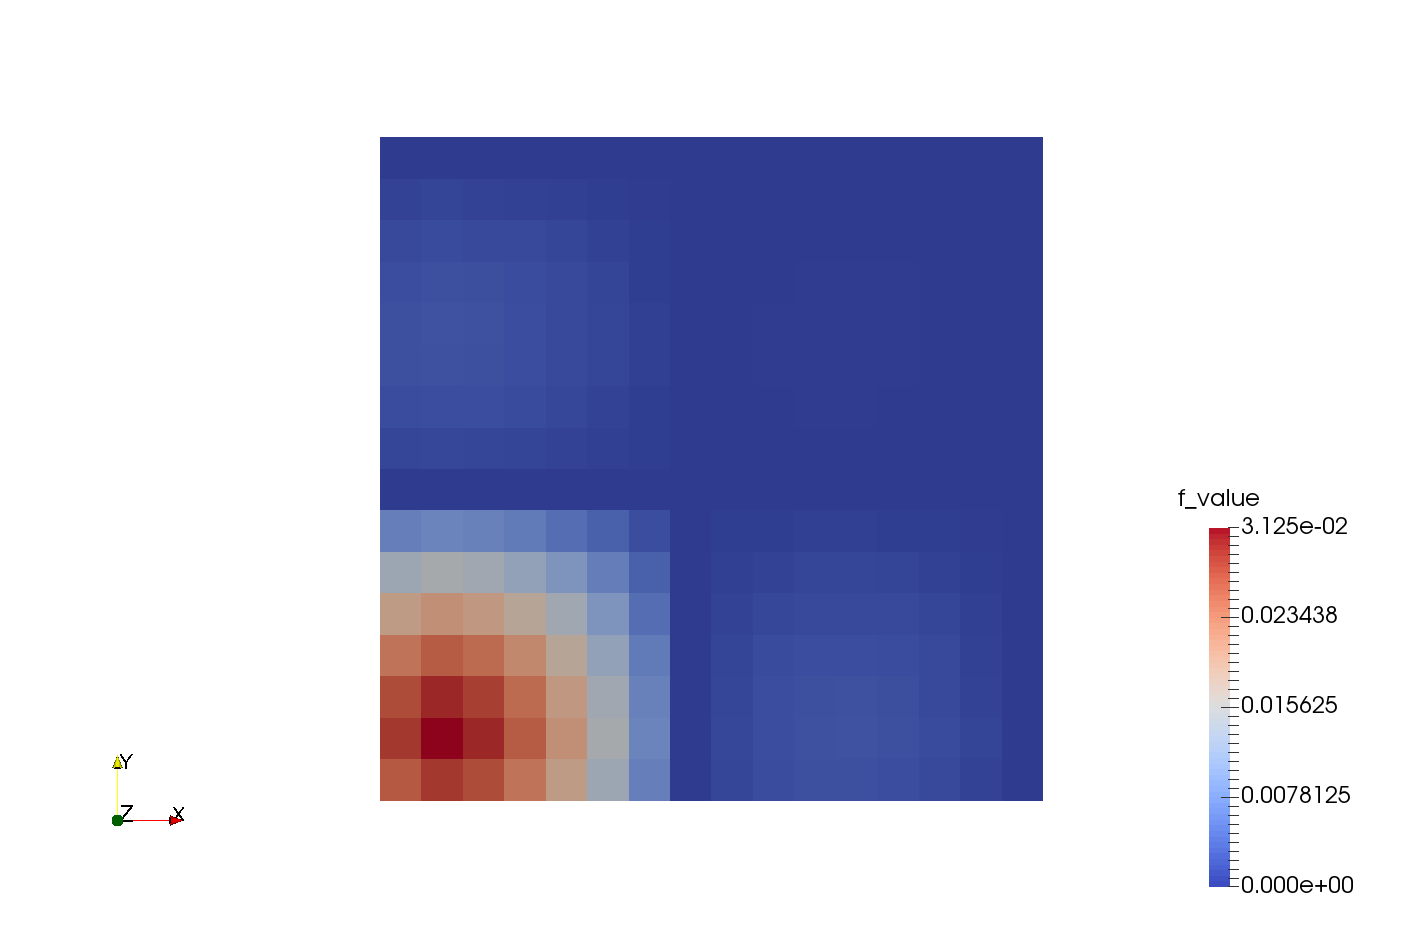
\includegraphics[width =\textwidth]{/results/4/case3-adaptive-before-refinement.png}
	    %\vspace{3em}
		\centering
        \caption{case 3 before refinement}
        \label{fig:AdaptiveCase3Before}
    \end{subfigure} 
    \begin{subfigure}[b]{0.49\textwidth}    
	    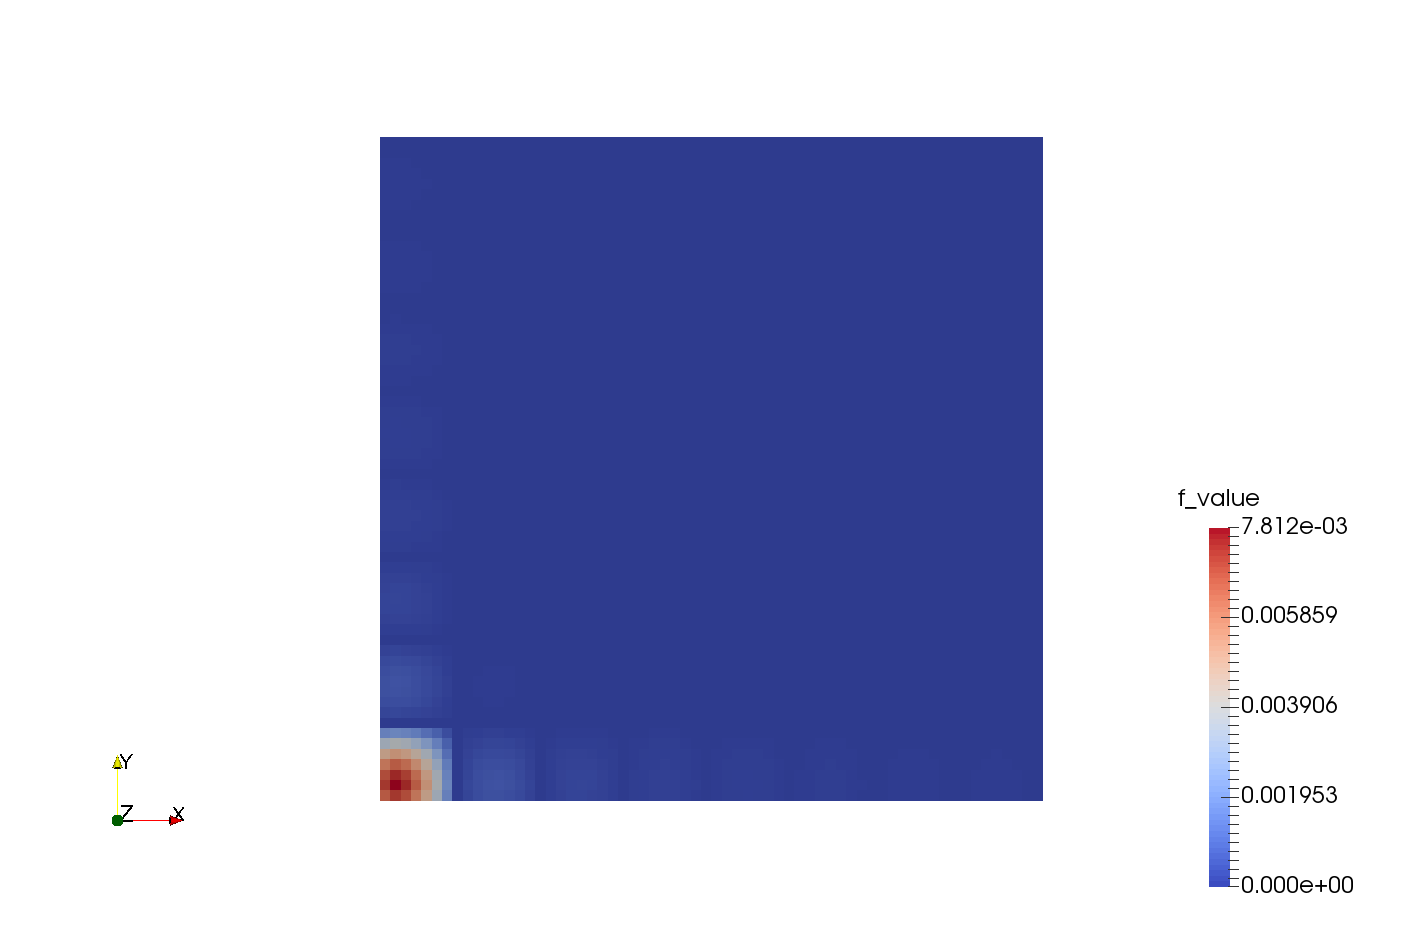
\includegraphics[width =\textwidth]{/results/4/case3-adaptive-after-refinement.png}
		\centering    
	 \caption{case 3 after refinement}
       \label{fig:AdaptiveCase3After}
    \end{subfigure} 
    \caption{Case 3 before and after refinement}
    \label{fig:AdaptiveCase3}
\end{figure}

%4adaptive case 4: before refinement and after refinement together
\begin{figure}[h]
	\centering
    \begin{subfigure}[b]{0.49\textwidth}
	    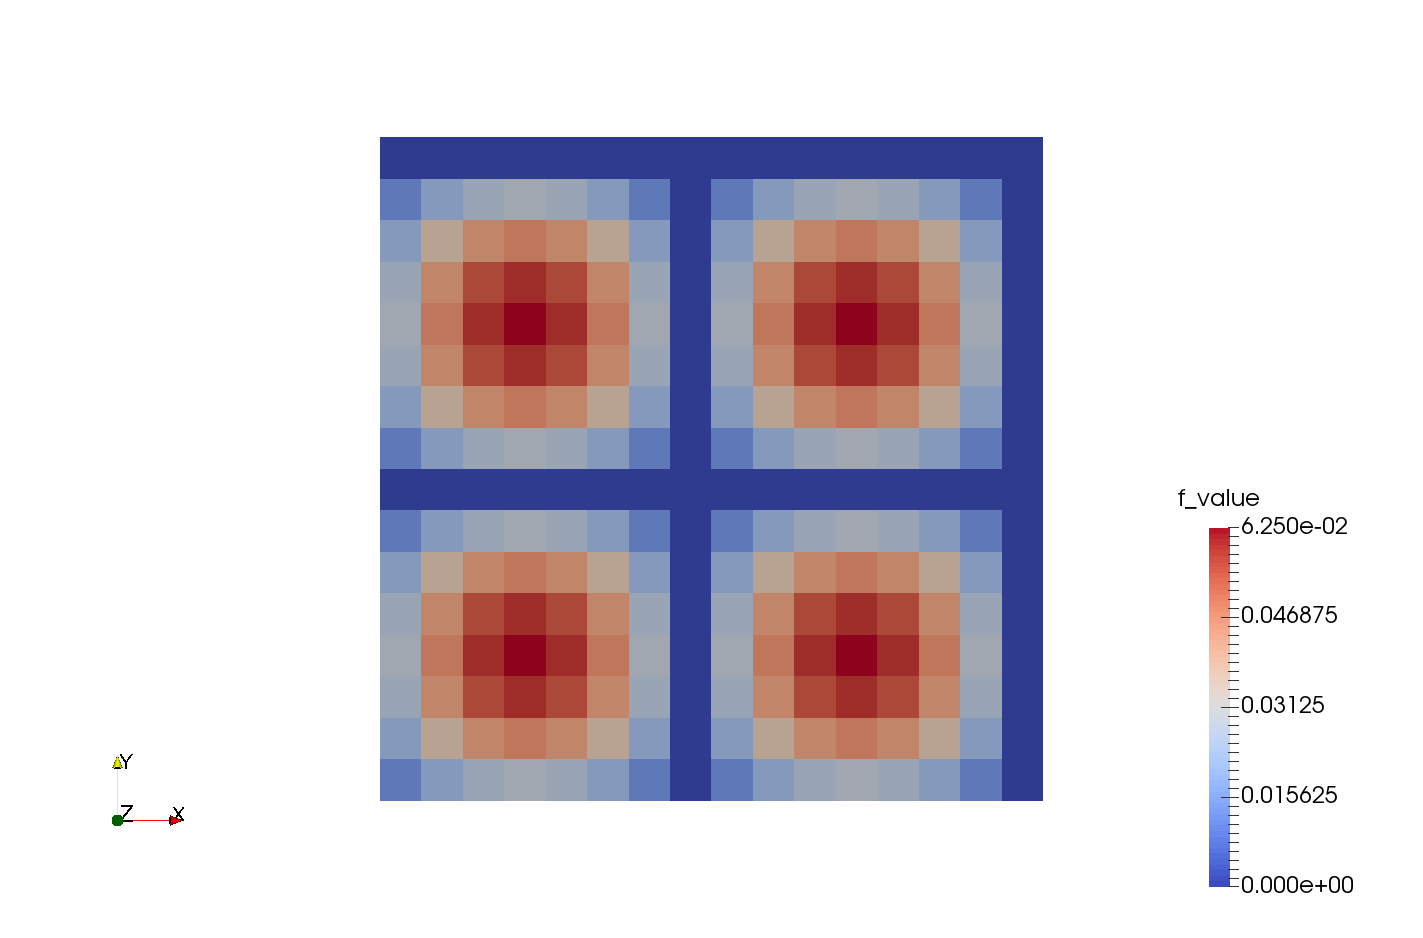
\includegraphics[width =\textwidth]{/results/4/case4-adaptive-before-refinement.png}
	    %\vspace{3em}
		\centering
        \caption{case 4 before refinement}
        \label{fig:AdaptiveCase4Before}
    \end{subfigure} 
    \begin{subfigure}[b]{0.49\textwidth}    
	    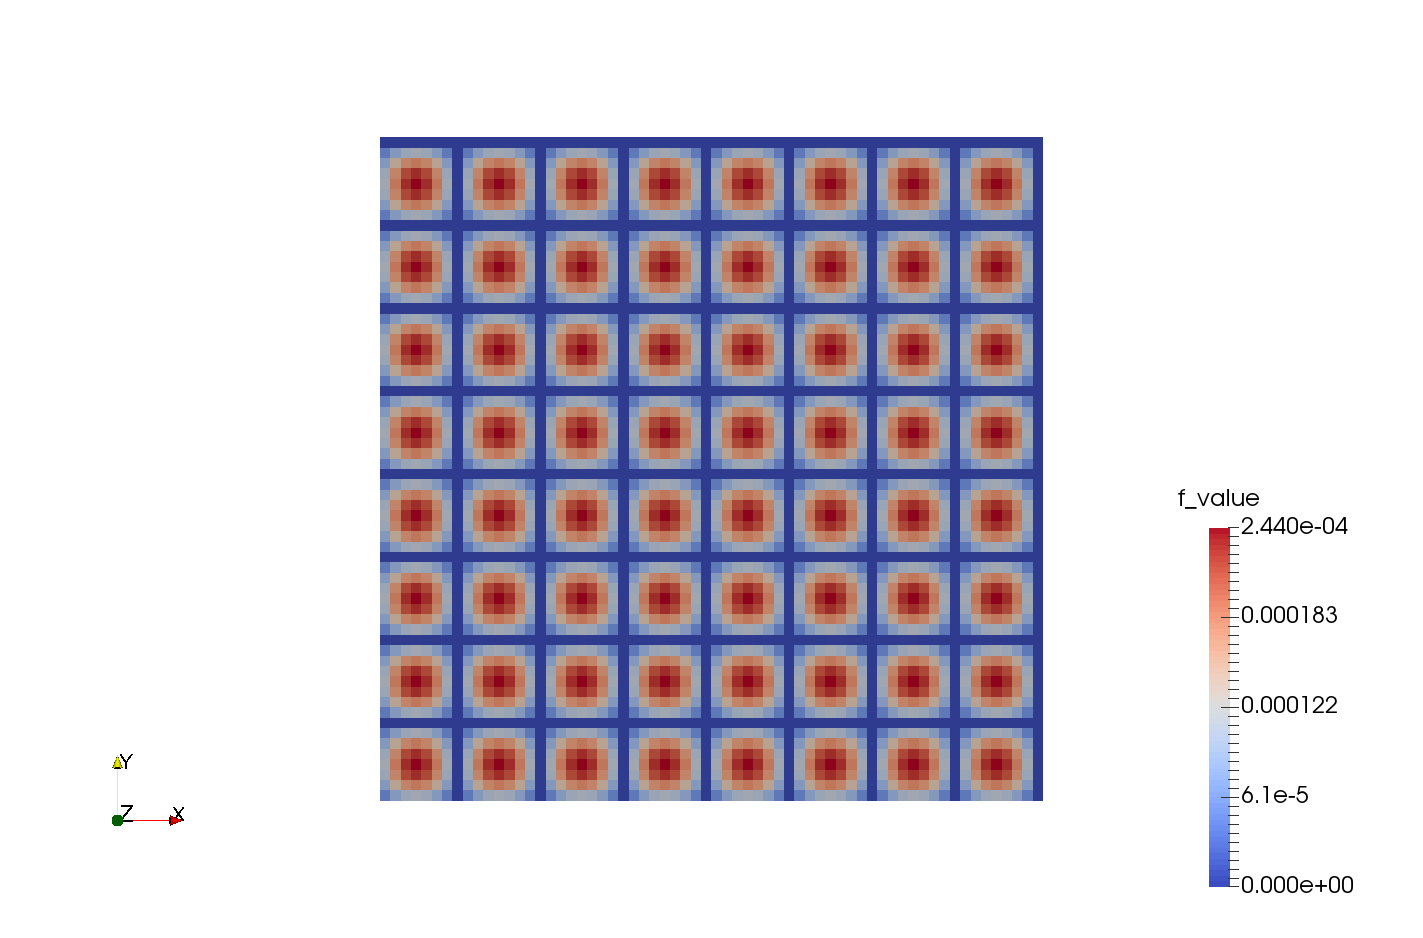
\includegraphics[width =\textwidth]{/results/4/case4-adaptive-after-refinement.png}
		\centering    
	 \caption{case 4 after refinement}
       \label{fig:AdaptiveCase4After}
    \end{subfigure} 
    \caption{Case 4 before and after refinement}
    \label{fig:AdaptiveCase4}
\end{figure}


It is important to point out the necessity of visualizing the error in the solution because from the solution images, the difference is hard to distinguish with human eye.

\section{Error and Accuracy}
In the last section the error is visualized in unit square simply because it doesn't make sense to just give one total error value for a special schemes. The difference here is to have multiple refinement levels performed in a loop/recursive way and then check how the total error acts. Based on arguments in literature a logarithmic behavior is expected. Key factors in the implemented code which are at play are threshold for the error and the level of refinement. Based on them some other schemes imagined here are as follow:
\begin{enumerate}
\item Threshold independent, refinement level changing.
\item Threshold changing, refinement level constant.
\end{enumerate}
The reason for these two scheme is that the results should be separated and based on the factors at play. Figures \ref{fig:ErrorRefinementLevel} and \ref{fig:ErrorThreshod} show the resulting error graphs for cases 2 to 4.

%5figure error threshold independent
%5figure refinement level constant

\begin{figure}[h]
	\centering
	    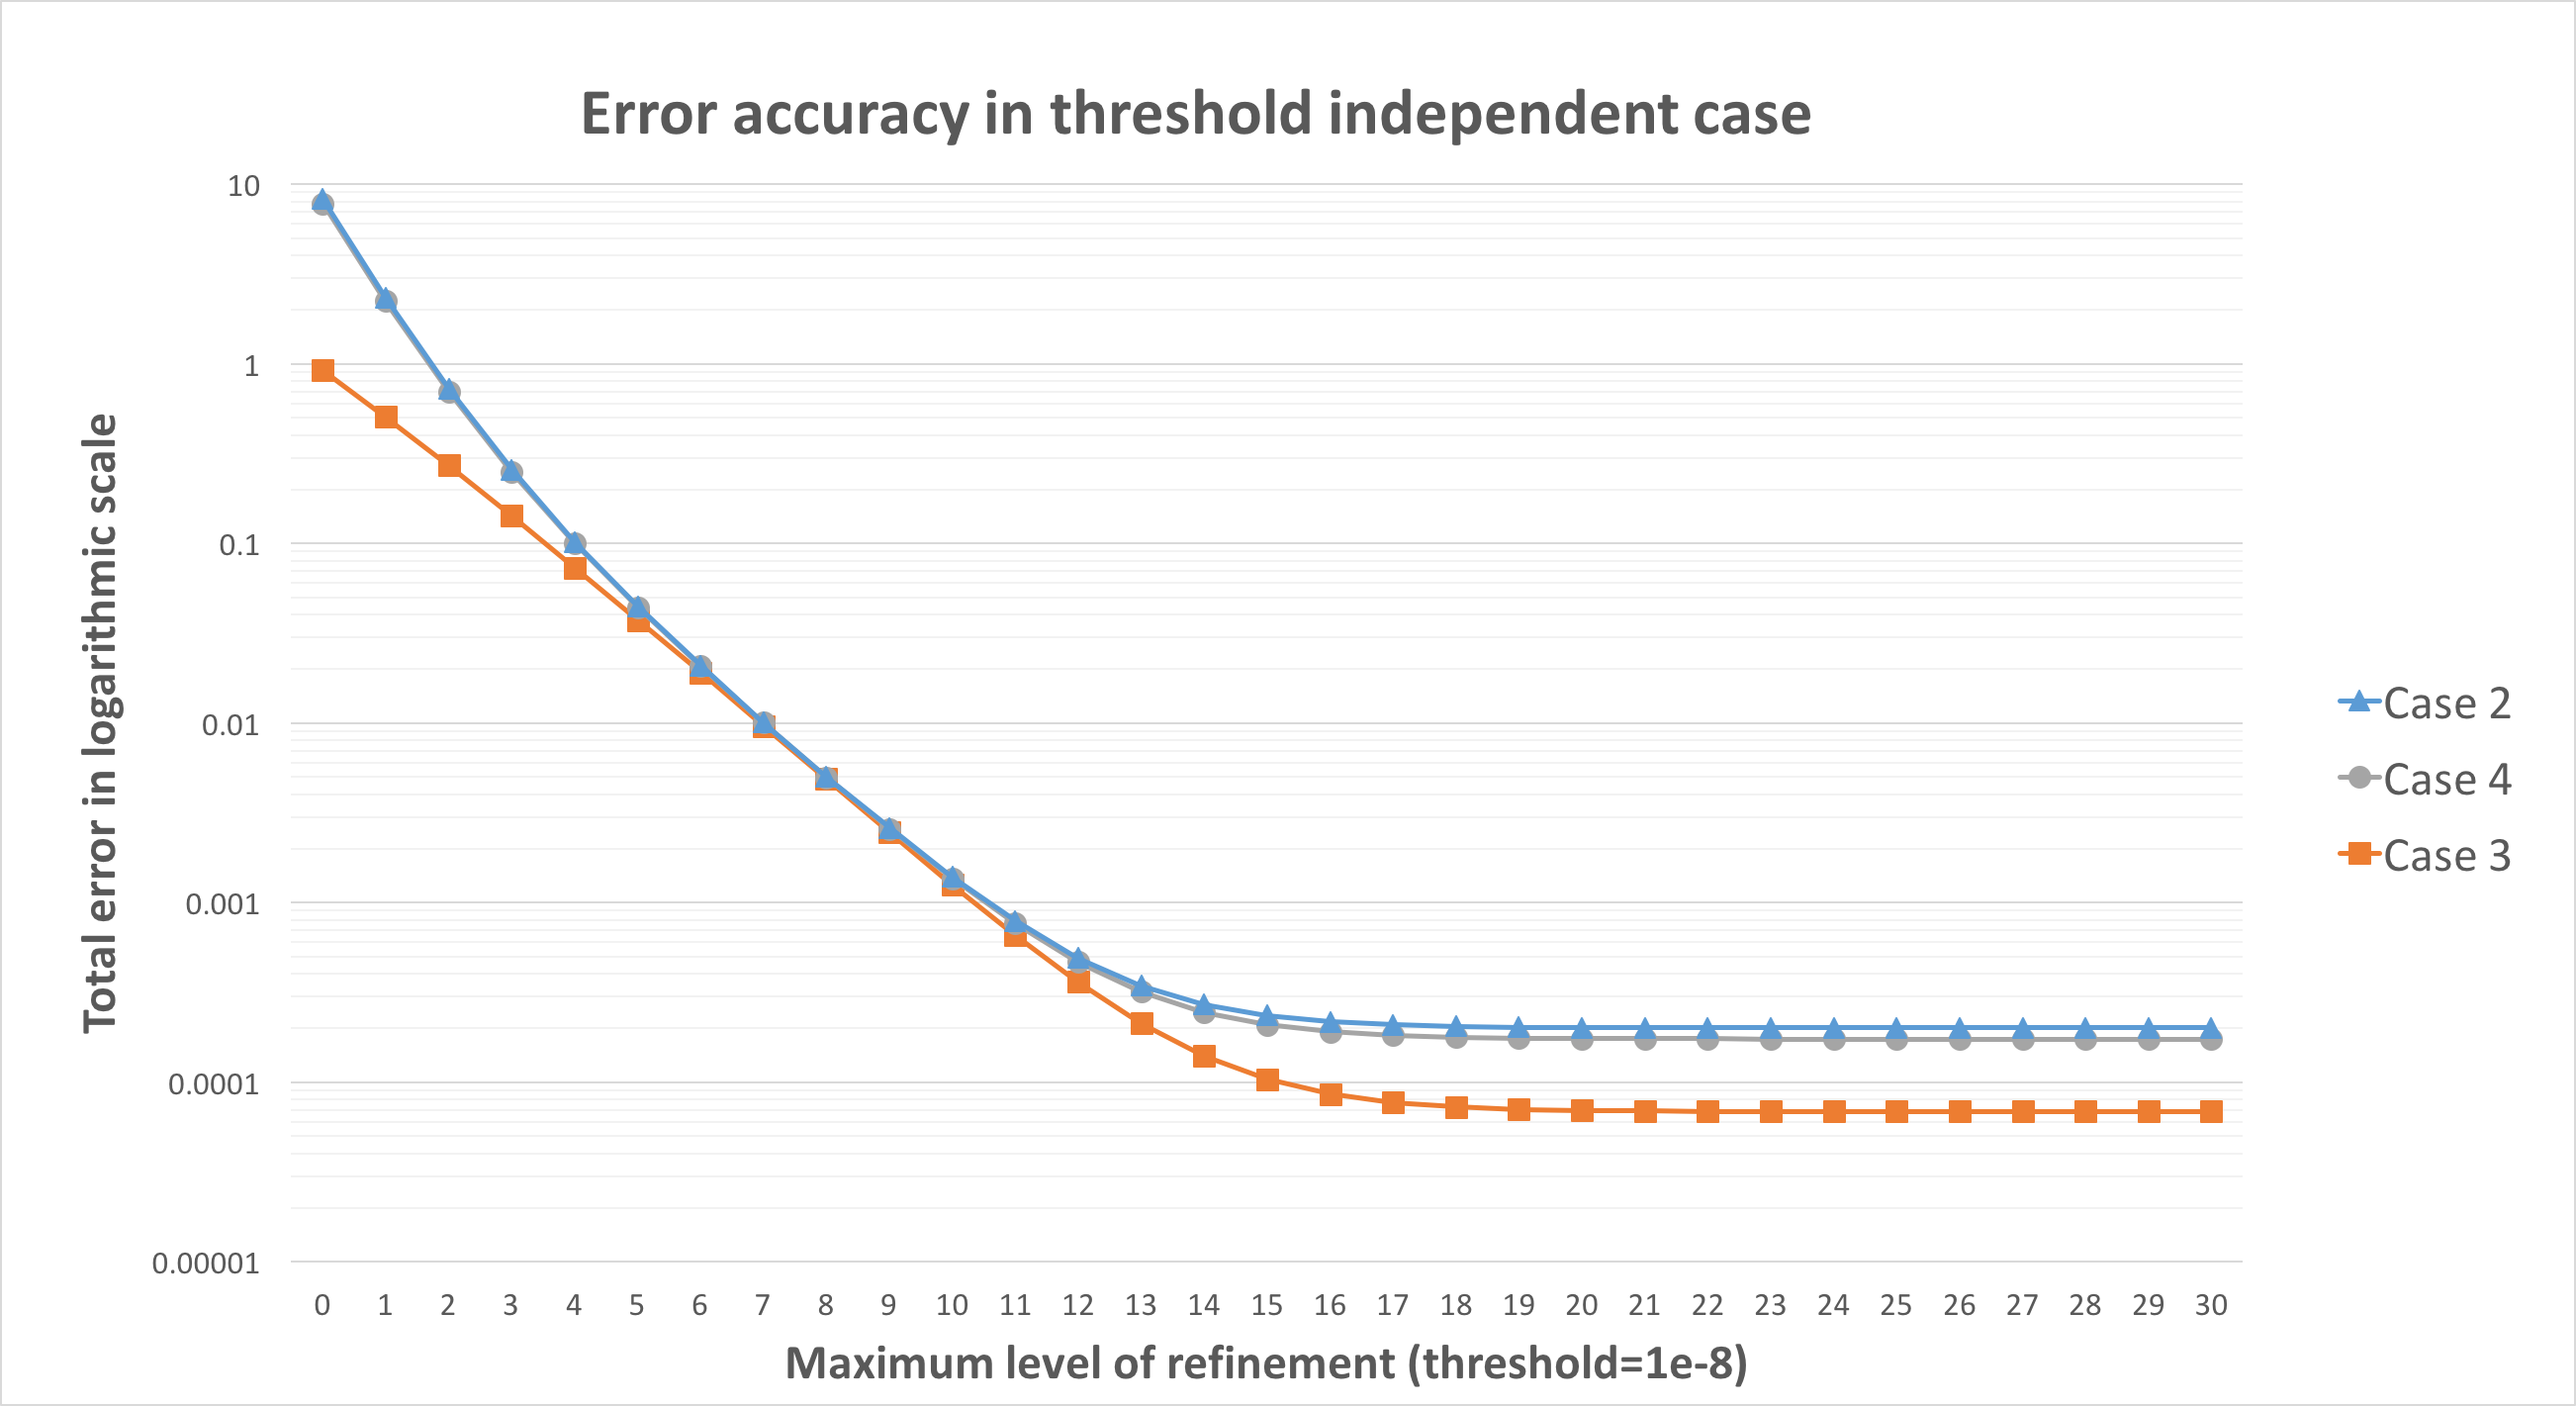
\includegraphics[width =\textwidth]{/results/5/Error-RefinementLevel.png}
		\centering    
	 \caption{Error-RefinementLevel}
       \label{fig:ErrorRefinementLevel}
\end{figure}

\begin{figure}[h]
	\centering
	    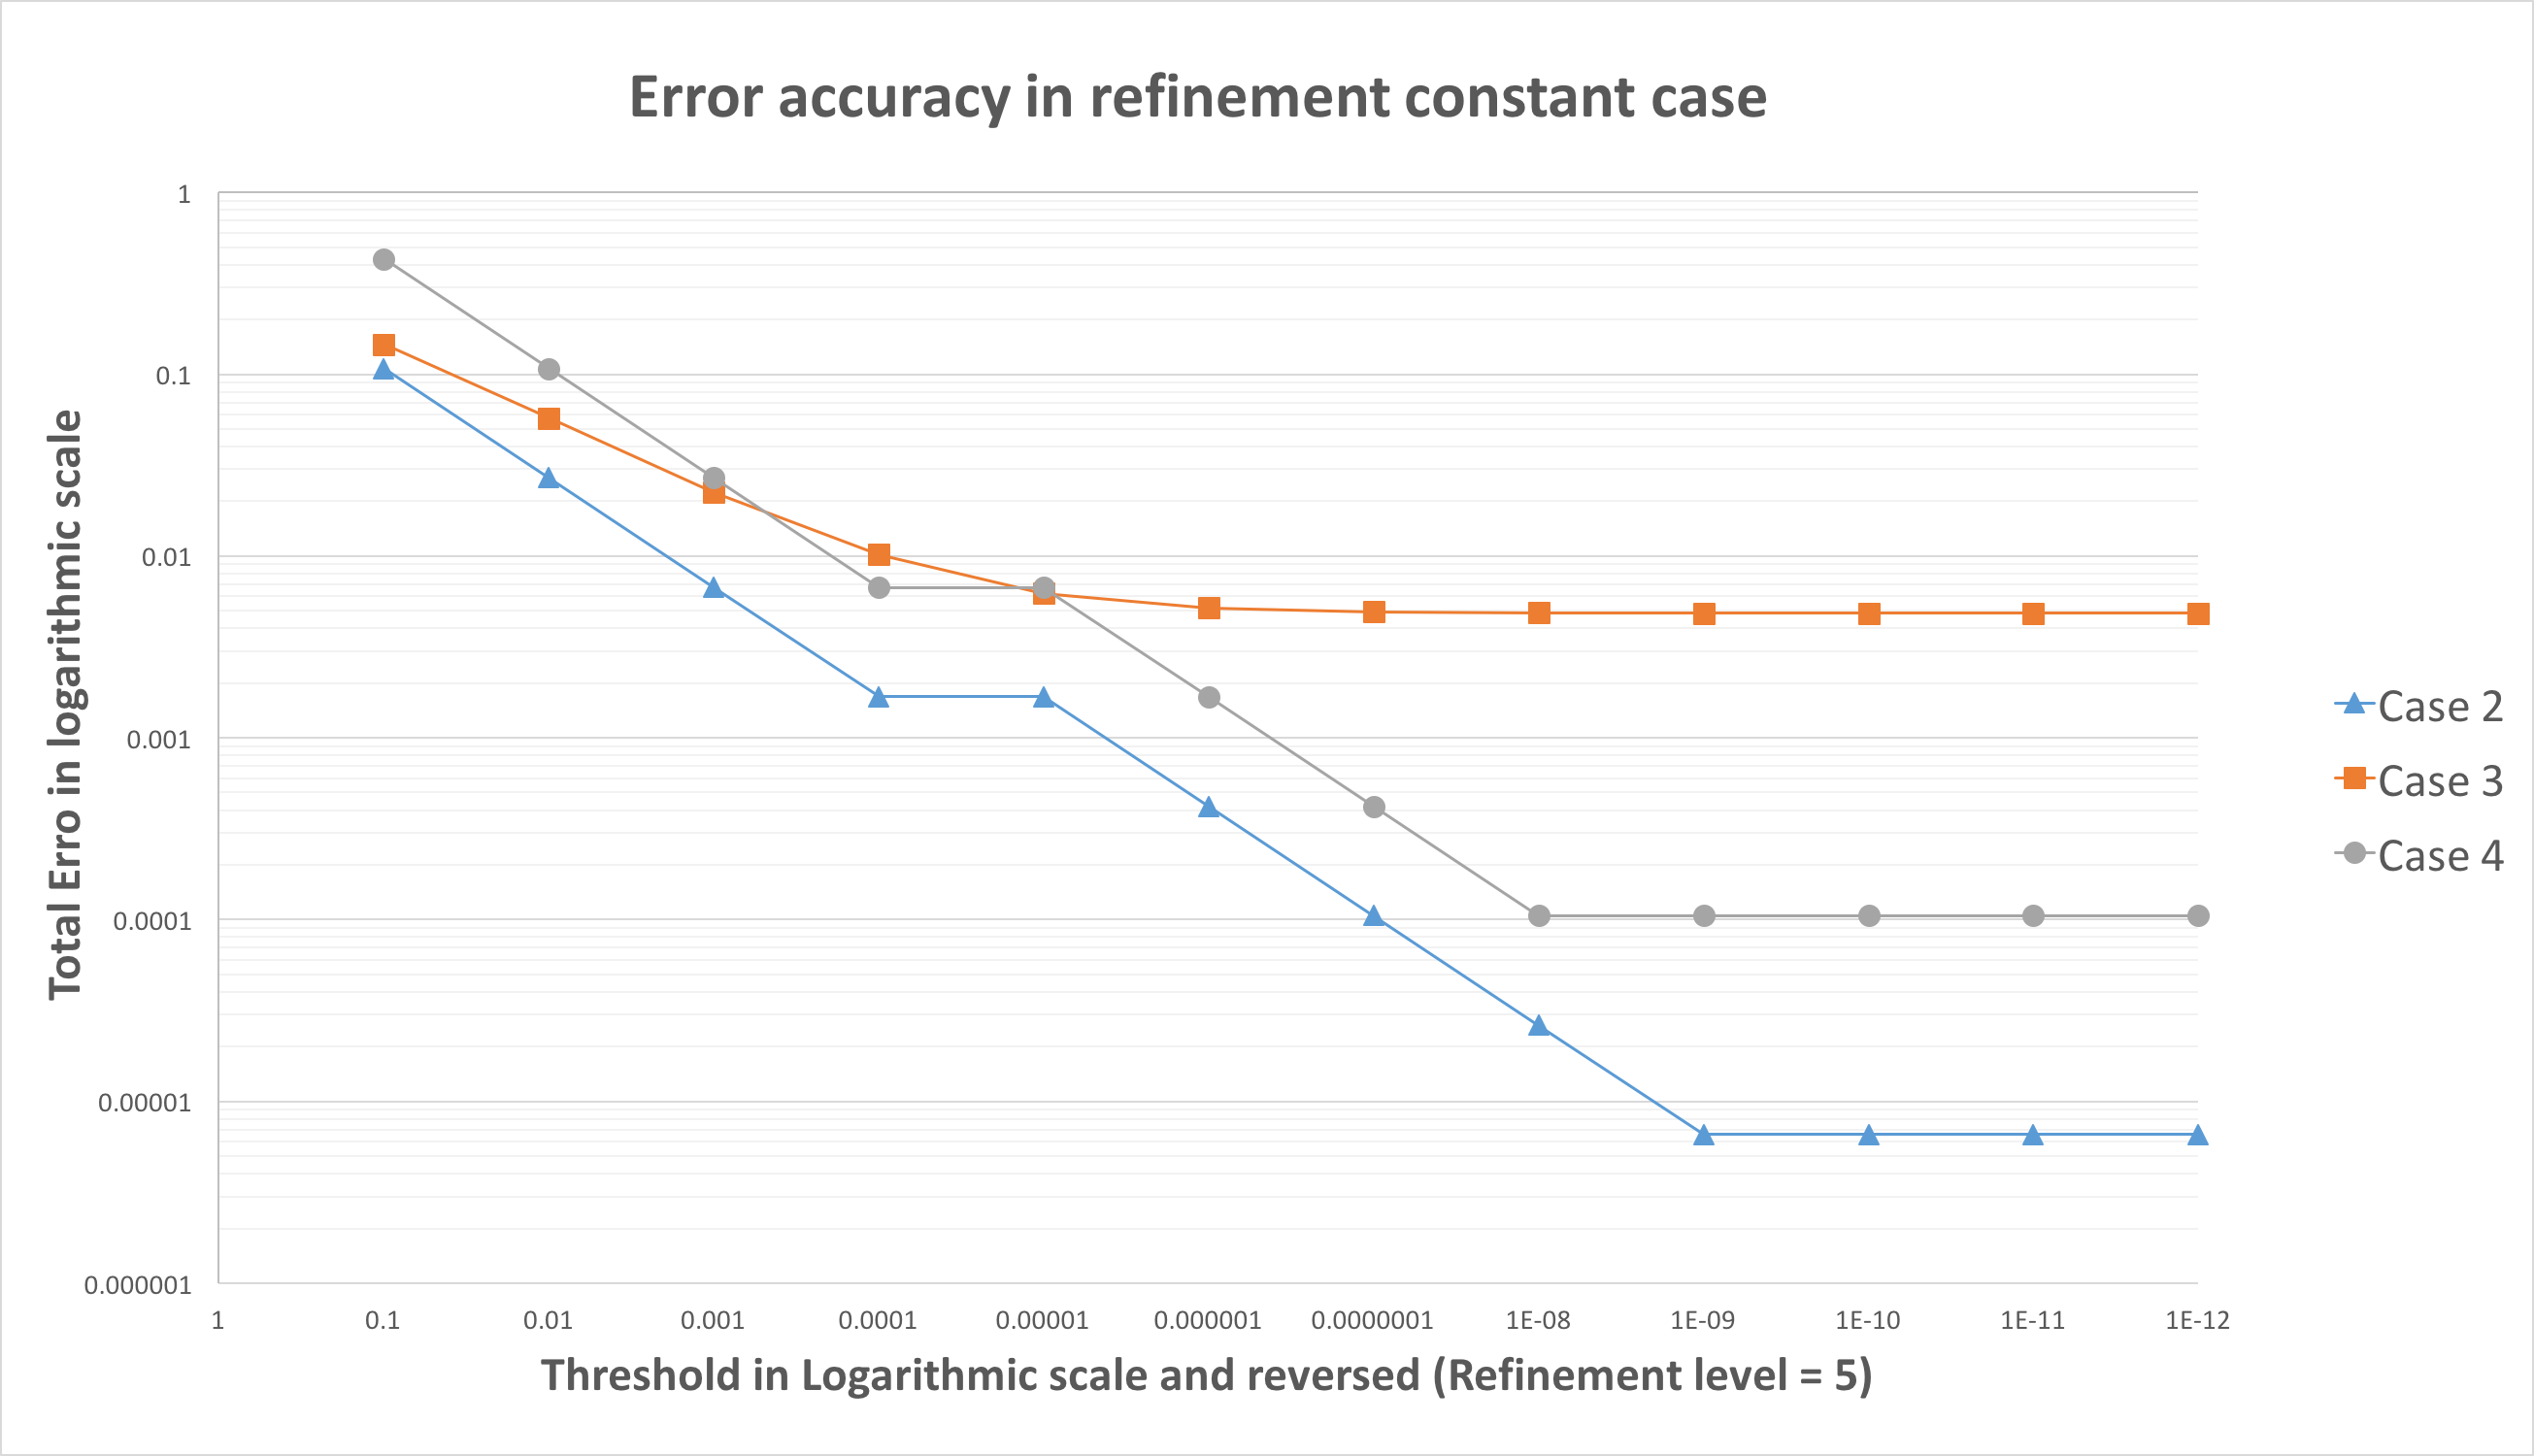
\includegraphics[width =\textwidth]{/results/5/Error-Threshod.png}
		\centering    
	 \caption{Error-Threshold}
       \label{fig:ErrorThreshod}
\end{figure}

As expected, the logarithmic error in both cases decreases with an increase in the level of mesh refinement and becomes constant after one point. It highlights the fact that the mesh independence is achieved in both cases and the results are free from the effect of the mesh refinement. Comparison of figures \ref{fig:ErrorRefinementLevel} and \ref{fig:ErrorThreshod} for case 2 shows much higher error in the threshold-independent approach and a significantly lower error in the refinement-constant approach. The reason is due to the specific definition of the function, in which only a small subsection is relevant for mesh-refinement. As the threshold-independent approach is unable to focus on a specific subsection, the resulting error is higher by a factor of 10 compared to the refinement-constant approach.





